\documentclass[12pt]{article}
\usepackage{graphicx}
\usepackage{mathptmx}
\usepackage{etoolbox}
\usepackage{ragged2e}
\usepackage{tabularx}
\usepackage{hyperref}
\usepackage{geometry}
\usepackage{etoolbox}
\usepackage{float}
\usepackage[acronym]{glossaries}
\makeatletter
% \patchcmd{<cmd>}{<search>}{<replace>}{<success>}{<failure>}
\patchcmd{\@makechapterhead}{\huge}{\large}{}{}% for \chapter
\patchcmd{\@makechapterhead}{\Huge}{\large}{}{}% for \chapter
\patchcmd{\@makeschapterhead}{\Huge}{\large}{}{}% for \chapter*
\tolerance=1
\emergencystretch=\maxdimen
\hyphenpenalty=10000
\hbadness=10000
\geometry{a4paper,total={170mm,257mm},left=20mm,top=20mm}

\patchcmd{\thebibliography}{\section*{\refname}}{}{}{}

% Acronyms
% abbreviations:
\newacronym{nfc}{NFC}{Near Field Communication}
\newacronym{ocr}{OCR}{Optical Character Recognition}
\newacronym{rfid}{RFID}{Radio-Frequency Identification}

% nomenclature:
\newglossaryentry{NFC}{
  name = NFC,
  description = is a communication protocol for communication between two electronic devices over a distance of $4 cm$,
}
\newglossaryentry{keys}{
  name = keys,
  description = in NOSQL keys are used to identify unique values
}
\newglossaryentry{geofence}{
  name = geofence,
  description = a virtual boundary triggered when an entity enters/leaves
}
\newglossaryentry{RFID}{
  name = RFID,
  description = is wireless communcation via tags and readers like \textit{NFC tags}
}

\makenoidxglossaries
\begin{document}
\begin{titlepage}
    \centering
    
\includegraphics[width=10cm]{manipal.png}
    
    \vskip7.4cm
    AT Lab Report\\
    B.Tech IT 6$^{th}$ Semester\\
    \vskip1cm
    {\bfseries\Large
        Mess Management App - Don’t Starve\\
    }
    \vskip1cm
    \textit{Submitted by}
    \vskip0.5cm
    \begin{tabularx}{0.8\textwidth} {>{\raggedright\arraybackslash}X>{\raggedleft\arraybackslash}X}
        Siddhant Dorman & 180911142 \\
        Nikesh Kumar & 180911202 \\
        Anjali Singh & 180911274
    \end{tabularx}
    \vfill
\end{titlepage}
\thispagestyle{empty}
\newpage

\tableofcontents
\thispagestyle{empty}
\newpage

\pagenumbering{roman}
% ---------------- Abstract ----------------
\section*{\LARGE{Abstract}}
\addcontentsline{toc}{section}{\protect\numberline{}Abstract}
{\justify
This project aims to create an efficient mess management application that addresses various problems as discussed ahead. \par
Food tokens in FC2 work on the principle of \gls{rfid}, which has several downfalls, including loss and theft of mess cards. To curb this problem, the app will use an inbuilt \gls{nfc} to emit the identification for the user. Thus, it will render physical mess cards obsolete, replacing them with portable ones. \par
Another common issue faced frequently is excessive crowding, especially during the time of the pandemic. With the help of geofencing, users will observe the real-time crowd and choose a time best suitable for them. \par
Furthermore, the app will have other functionalities like accessing the daily mess menu.
}

% ---------------- Abbreviations ----------------
\section*{\LARGE{List of Abbreviations}}
\addcontentsline{toc}{section}{\protect\numberline{}List of Abbreviations}
\printnoidxglossary[type=\acronymtype,title=Acronyms,nonumberlist]
\printnoidxglossary[title=Description,nonumberlist]
\newpage

% ---------------- Introduction ----------------
\pagenumbering{arabic}
\section*{\LARGE{Introduction}}
\addcontentsline{toc}{section}{\protect\numberline{}Introduction}
COVID-19, overcrowding, and obsolete technology are the reasons for the existence of this project. The idea behind the project is to deal with the shortcomings as listed but on a smaller level, i.e., in food courts/messes. The Android application, `Don\textquotesingle t Starve' aims to provide a smooth and effortless experience coupled with some guise of safety from COVID-19 in food courts to the user.\par \vskip0.3cm
This application will allow users to register and get verified (more information under Product Functions) and access mess resources with ease. There is a provision of an `editable' (by the admin) daily menu. This is to provide the students with a list of delicacies that will be served on that day. Furthermore, this will reduce the usage of paper as printing menus daily would be unnecessary.\par \vskip0.3cm
Mess cards are subject to theft or loss. Furthermore, carrying them with oneself is also a task sometimes. One might forget to take their cards with them during meals. Since everyone brings their phone everywhere with them, the ideal solution would be to amalgamate the cards, i.e., the identifier, with phones. With technology like NFC, mess cards will become obsolete, and the process of procuring food tokens will be trouble-free.\par \vskip0.3cm
Food courts are incredibly crowded at certain times. Given the current scenario and how critical social distancing is in today's world, the technology of Geofencing comes to the rescue. This feature will provide real-time data about the number of people in a particular geographical area, i.e., the food courts. Students can refer to the statistics and decide at what time they\textquotesingle d like to have their meals.\par \vskip0.3cm
The project will be able to provide a seamless experience to the users during the ongoing pandemic. It will also have a social and environmental impact simultaneously. The app helps eliminate the use of plastic for mess cards and provides a safe environment for students to have their meals without worrying about the crowds, thanks to geofencing. \par 
\begin{center}
    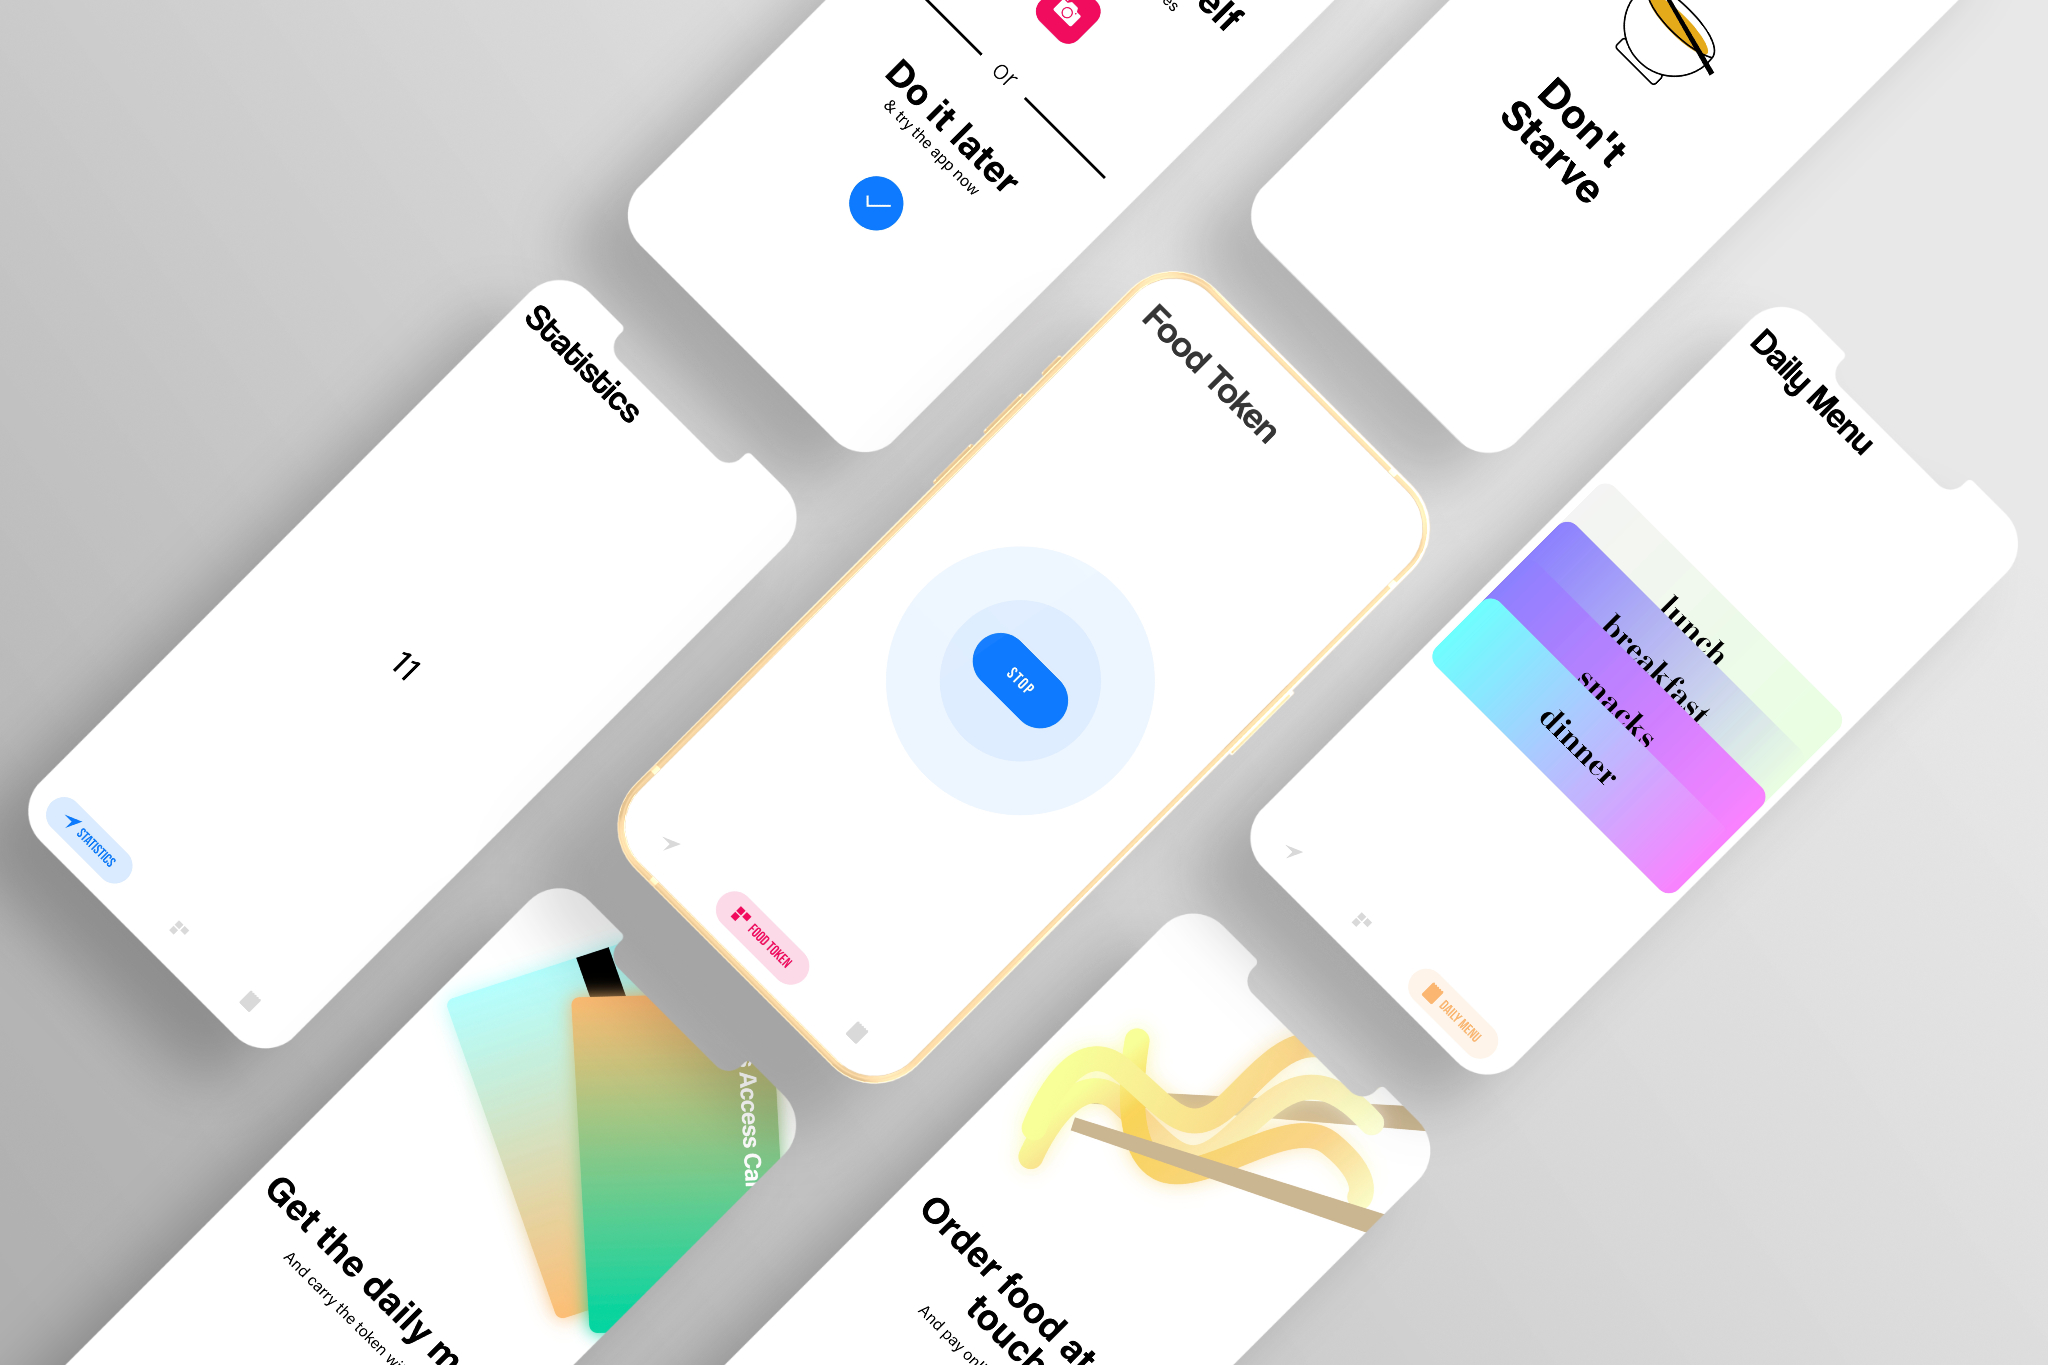
\includegraphics[width=\linewidth]{highlight.jpg}
\end{center}
\newpage

% ---------------- Language Description ----------------
\section*{\LARGE{Language Description}}
\addcontentsline{toc}{section}{\protect\numberline{}Language Description}

{\justify
Most of the project has primarily been coded in \textit{Java} in the IDE provided by Android Studio. Our project comprises two parts: the application \& the Console. The back-end is hosted on Firebase, which has been connected to both entities of our project. Development related to the mobile application has been done entirely on \textit{Java} with XML Designs, fonts and static images to serve the application. The Console have been made using \textit{React JS}, a JavaScript framework that has been hosted on GitHub pages and connects users to perform back-end changes without needing to login to Firebase.
}
\vskip1cm
\begin{figure}[H]
    \begin{minipage}{0.47\textwidth}
      \centering
      
\includegraphics[width=\linewidth]{slice1.png}
      \caption{Language distribution of Application}\label{Fig:Data1}
    \end{minipage}\hfill
    \begin{minipage}{0.47\textwidth}
      \centering
      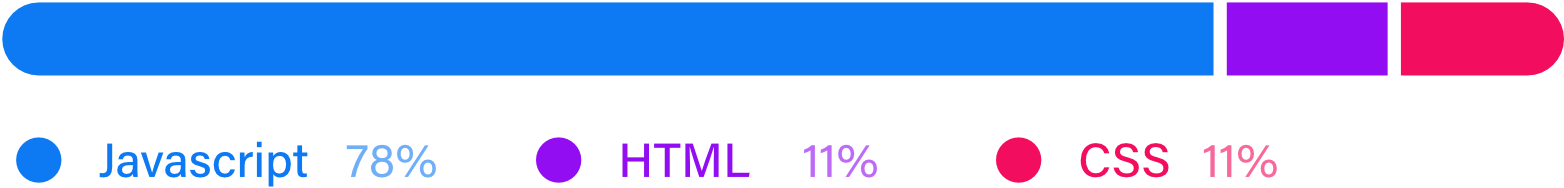
\includegraphics[width=\linewidth]{slice2.png}\hspace{0.5cm}
      \caption{Language distribution of Web App}\label{Fig:Data2}
    \end{minipage}
\end{figure}

% ---------------- Backend Design ----------------
\section*{\LARGE{Database Description}}
\addcontentsline{toc}{section}{\protect\numberline{}Database Description}


\subsection*{Firebase}
\addcontentsline{toc}{subsection}{\protect\numberline{}Firebase}
{\justify
The backend has been hosted on Firebase and makes use of Firebase Realtime Database \& Firebase Storage. 
Firebase Realtime Database is a real-time NoSQL Cloud database that stores data as a JSON object, and ours comprises three keys to handle crowd data, menu data, and registered users. For simplicity of usage, the login system based on username and password has been scrapped to support one-time identification based on the registration number, name, and email id. When a user enters their data, they will be asked to verify themselves. This data will be pushed to the database. Geofencing connects to the crowd key to fetch real-time crowd numbers and provide them to the user. The console retrieves the menu data and allows the admin to make changes and push it back to the database, fetched by the user whenever they open the app. 
Firebase Storage is cloud storage like AWS S3 Bucket, where objects/blob objects can be stored/retrieved. Here we primarily store the photos submitted by the user for verification which the console can retrieve to verify the user.
}
\vskip1cm
\begin{figure}[H]
    \centering
    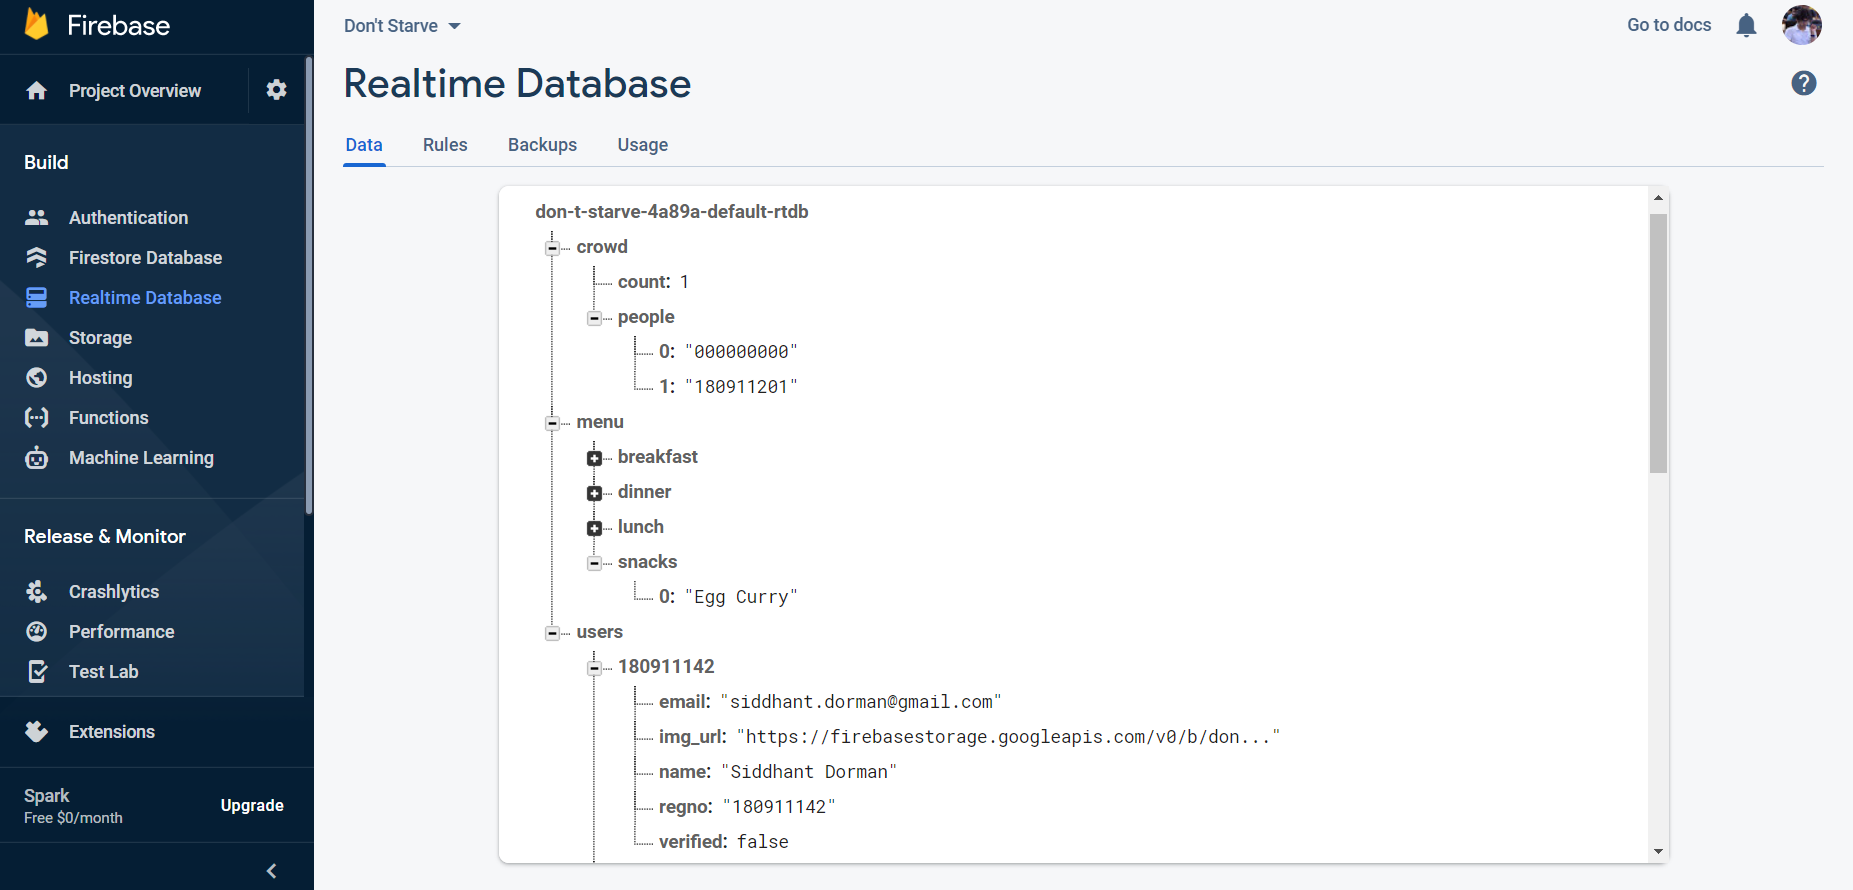
\includegraphics[width=0.7\linewidth]{rtdb.png}
    \caption{Firebase Realtime Database}
\end{figure}
\begin{figure}[H]
    \centering
    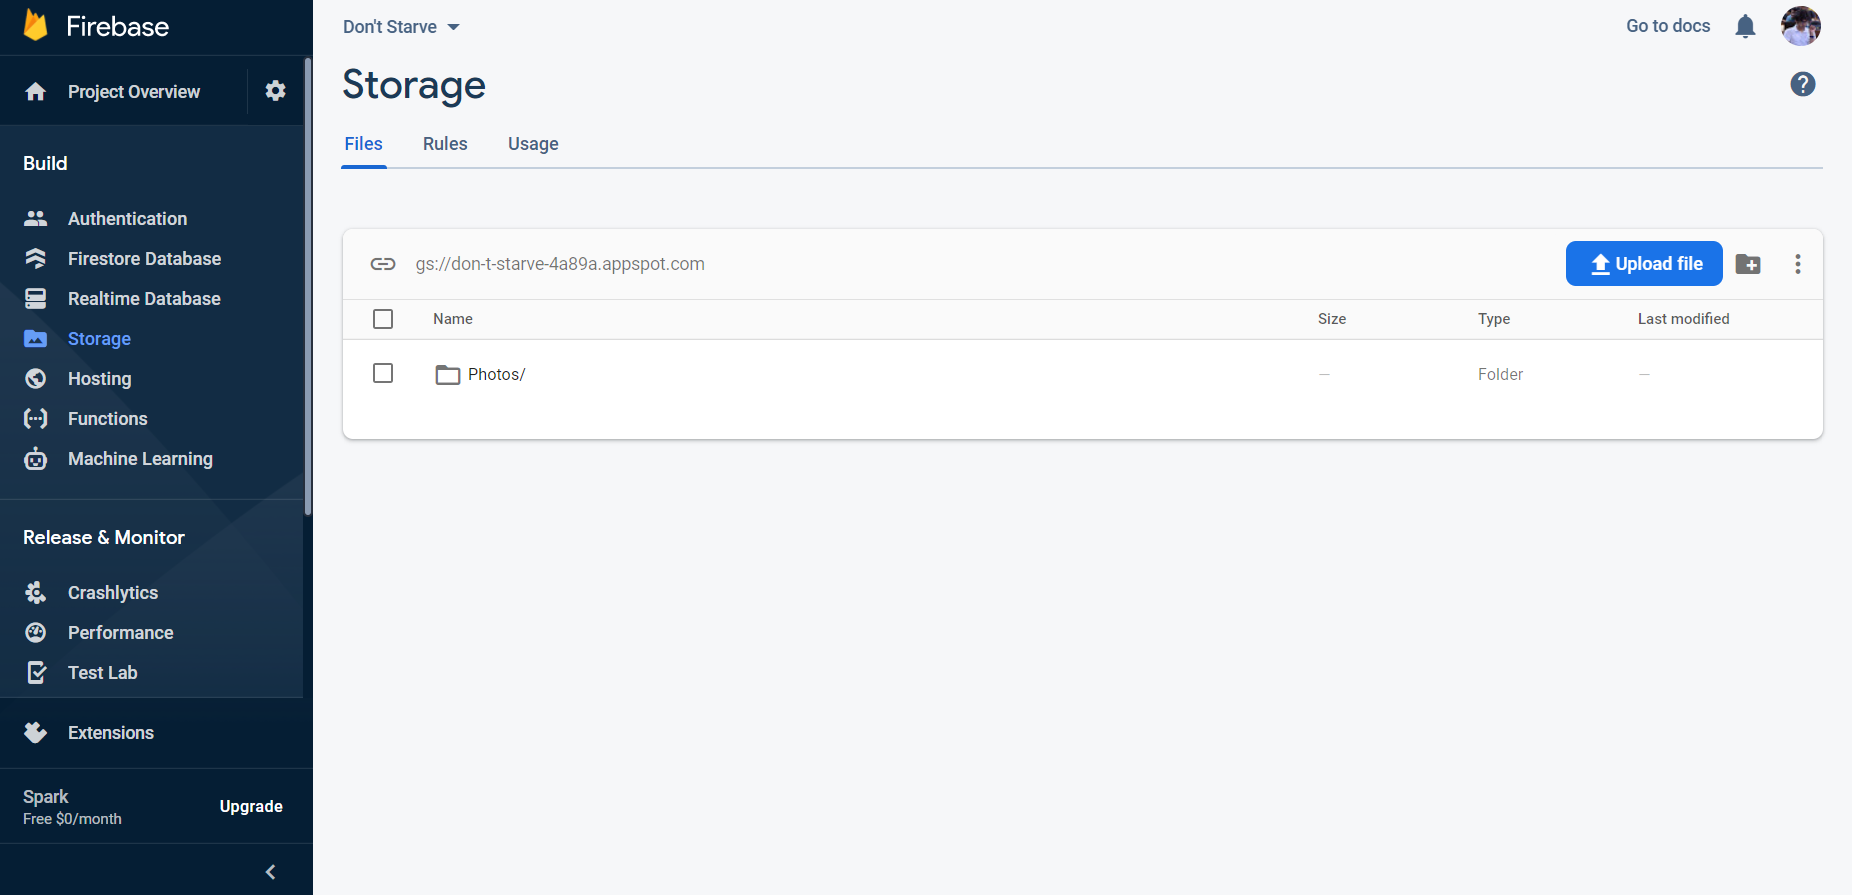
\includegraphics[width=0.7\linewidth]{storage.png}
    \caption{Firebase Storage}
\end{figure}

\subsection*{Console}
\addcontentsline{toc}{subsection}{\protect\numberline{}Console}
{\justify
The console handles the admin side and while it is not the backend, it can be termed as an extension of Firebase functionality. It enables the admin to approve users and to edit the daily menu which reflects changes on the Firebase side. It has been designed on React JS, a framework of Javascript which has been hosted on GitHub Pages of the same repository.
}
\begin{figure}[H]
    \centering
    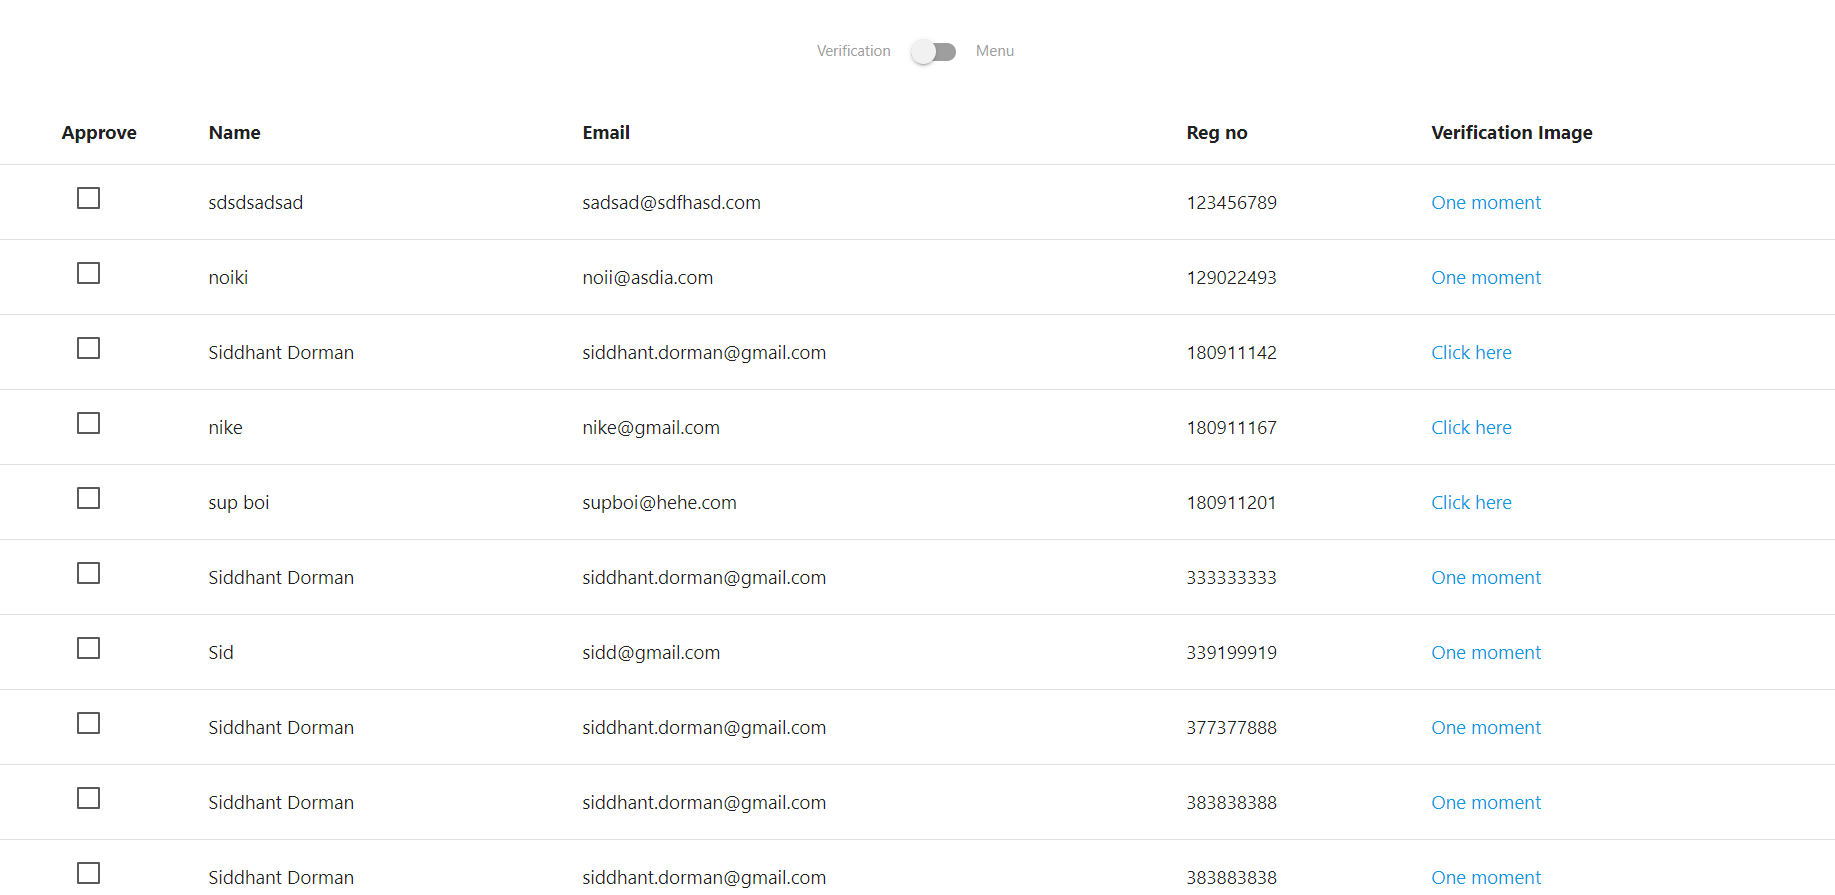
\includegraphics[width=0.7\linewidth]{verify.png}
    \caption{Console - Verification Tab}
\end{figure}
\begin{figure}[H]
    \centering
    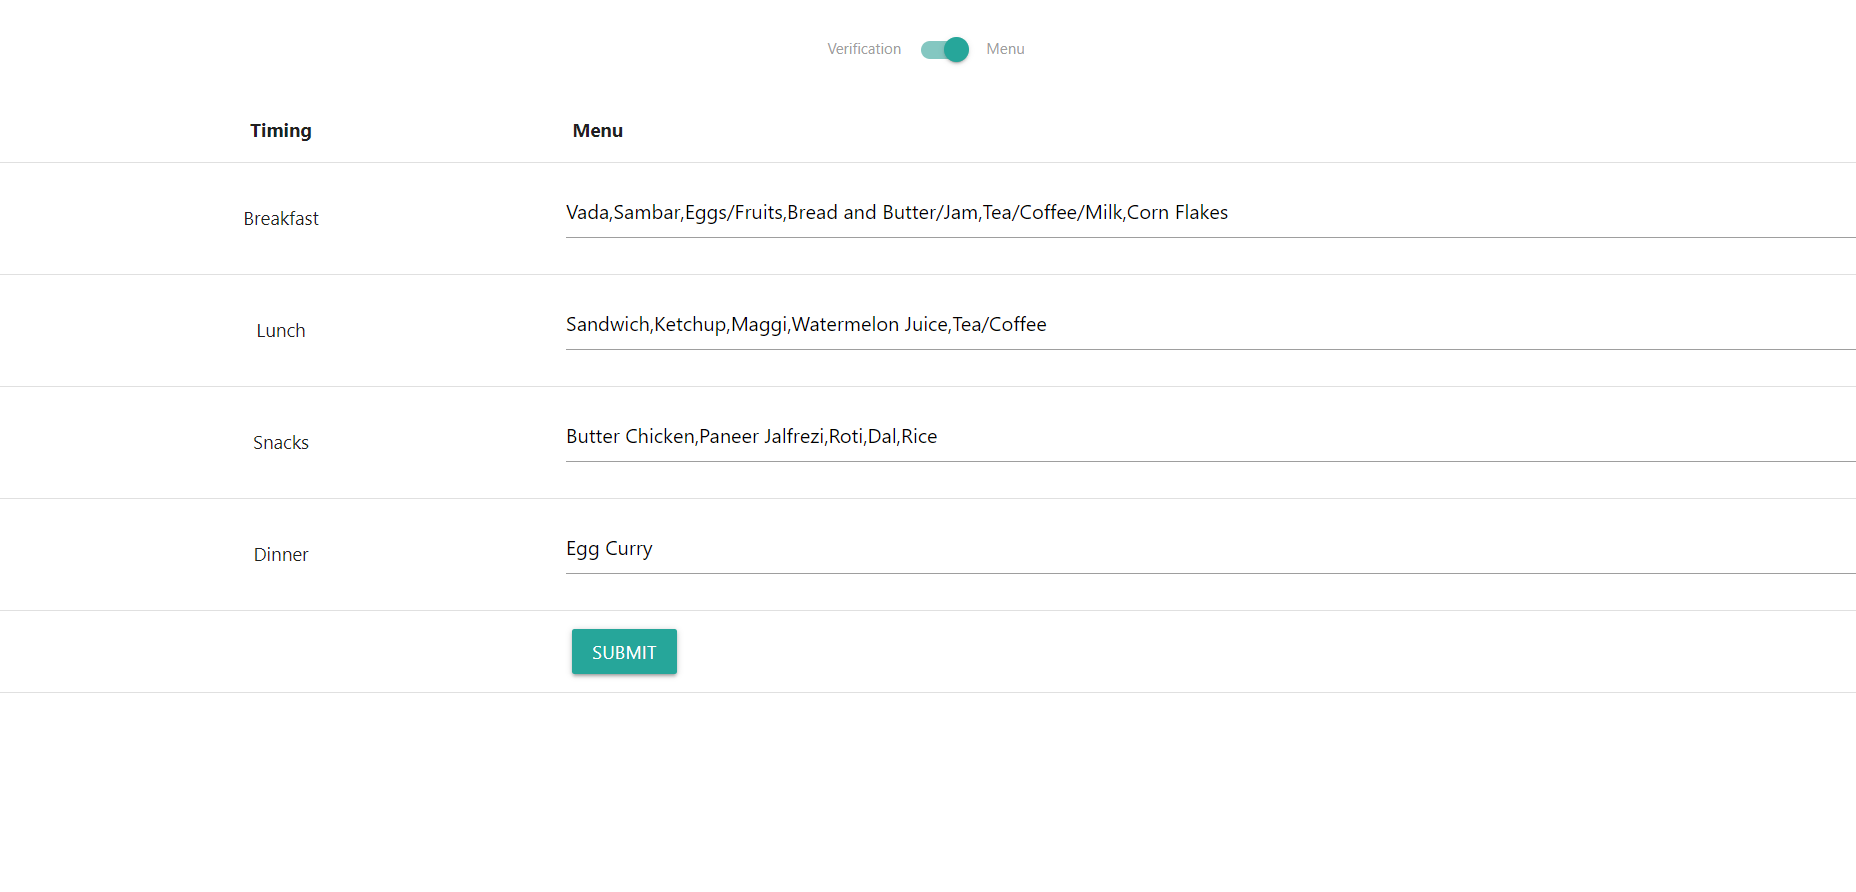
\includegraphics[width=0.7\linewidth]{food.png}
    \caption{Console - Menu Tab}
\end{figure}
\newpage

% ---------------- Project Description ----------------
\section*{\LARGE{Project Description}}
\addcontentsline{toc}{section}{\protect\numberline{}Project Description}
{\justify
The current pandemic has been unprecedented in its reach and depth of impact on the functioning of 
modern society. Social distancing is more important now than ever. We aim to provide an optimized 
solution to an otherwise unavoidable aspect of daily college life and some semblance of safety for the 
users. We aim to create an application providing real-time geofencing data of the food court, with contactless meal token
and menu features for usage by the students
}

% ---------------- Product Functions ----------------
\section*{\LARGE{Product Functions}}
\addcontentsline{toc}{section}{\protect\numberline{}Project Functions}

% \begin{itemize}
% \item 
\subsection*{Verify FC Users}
\addcontentsline{toc}{subsection}{\protect\numberline{}Verify FC Users}
{\justify This app makes use of inbuilt \gls{ocr} to identify the student from their identity card issued by MAHE. It will then compare it with the registration number and send it to the backend for storage. The user can also be verified via console in case of failure to identify, which serves as a fallback to the OCR.}

% \item 
\subsection*{Geofencing}
\addcontentsline{toc}{subsection}{\protect\numberline{}Geofencing}
{\justify Mess crowdings are a big issue which is why to tackle this we make use of android\textquotesingle s Geofencing. This feature makes use of background location access to detect any entry/exit in the area of \gls{geofence} to generate the crowd data. When triggered, it makes changes to the database which is then reflected in the application real-time.}

% \item 
\subsection*{Daily Menu}
\addcontentsline{toc}{subsection}{\protect\numberline{}Daily Menu}
{\justify One of the primary issues faced by the students is that they have no idea of the Daily Menu of the mess. This feature will allow the user to see the daily menu that is set by the admin from the Console.}

% \item 
\subsection*{NFC Food Token}
\addcontentsline{toc}{subsection}{\protect\numberline{}NFC Food Token}
{\justify Mess card are prone to physical damage, theft which can be tackled with the usage of virtual tokens. Currently this is a prototype to display how \gls{NFC} could be implemented as a method of Food Token in mess to validate user data with the machine.}
% \end{itemize}

\newpage

% ---------------- Product Designs ----------------
\section*{\LARGE{Designs}}
\addcontentsline{toc}{section}{\protect\numberline{}Designs}

\begin{figure}[H]
    \centering
    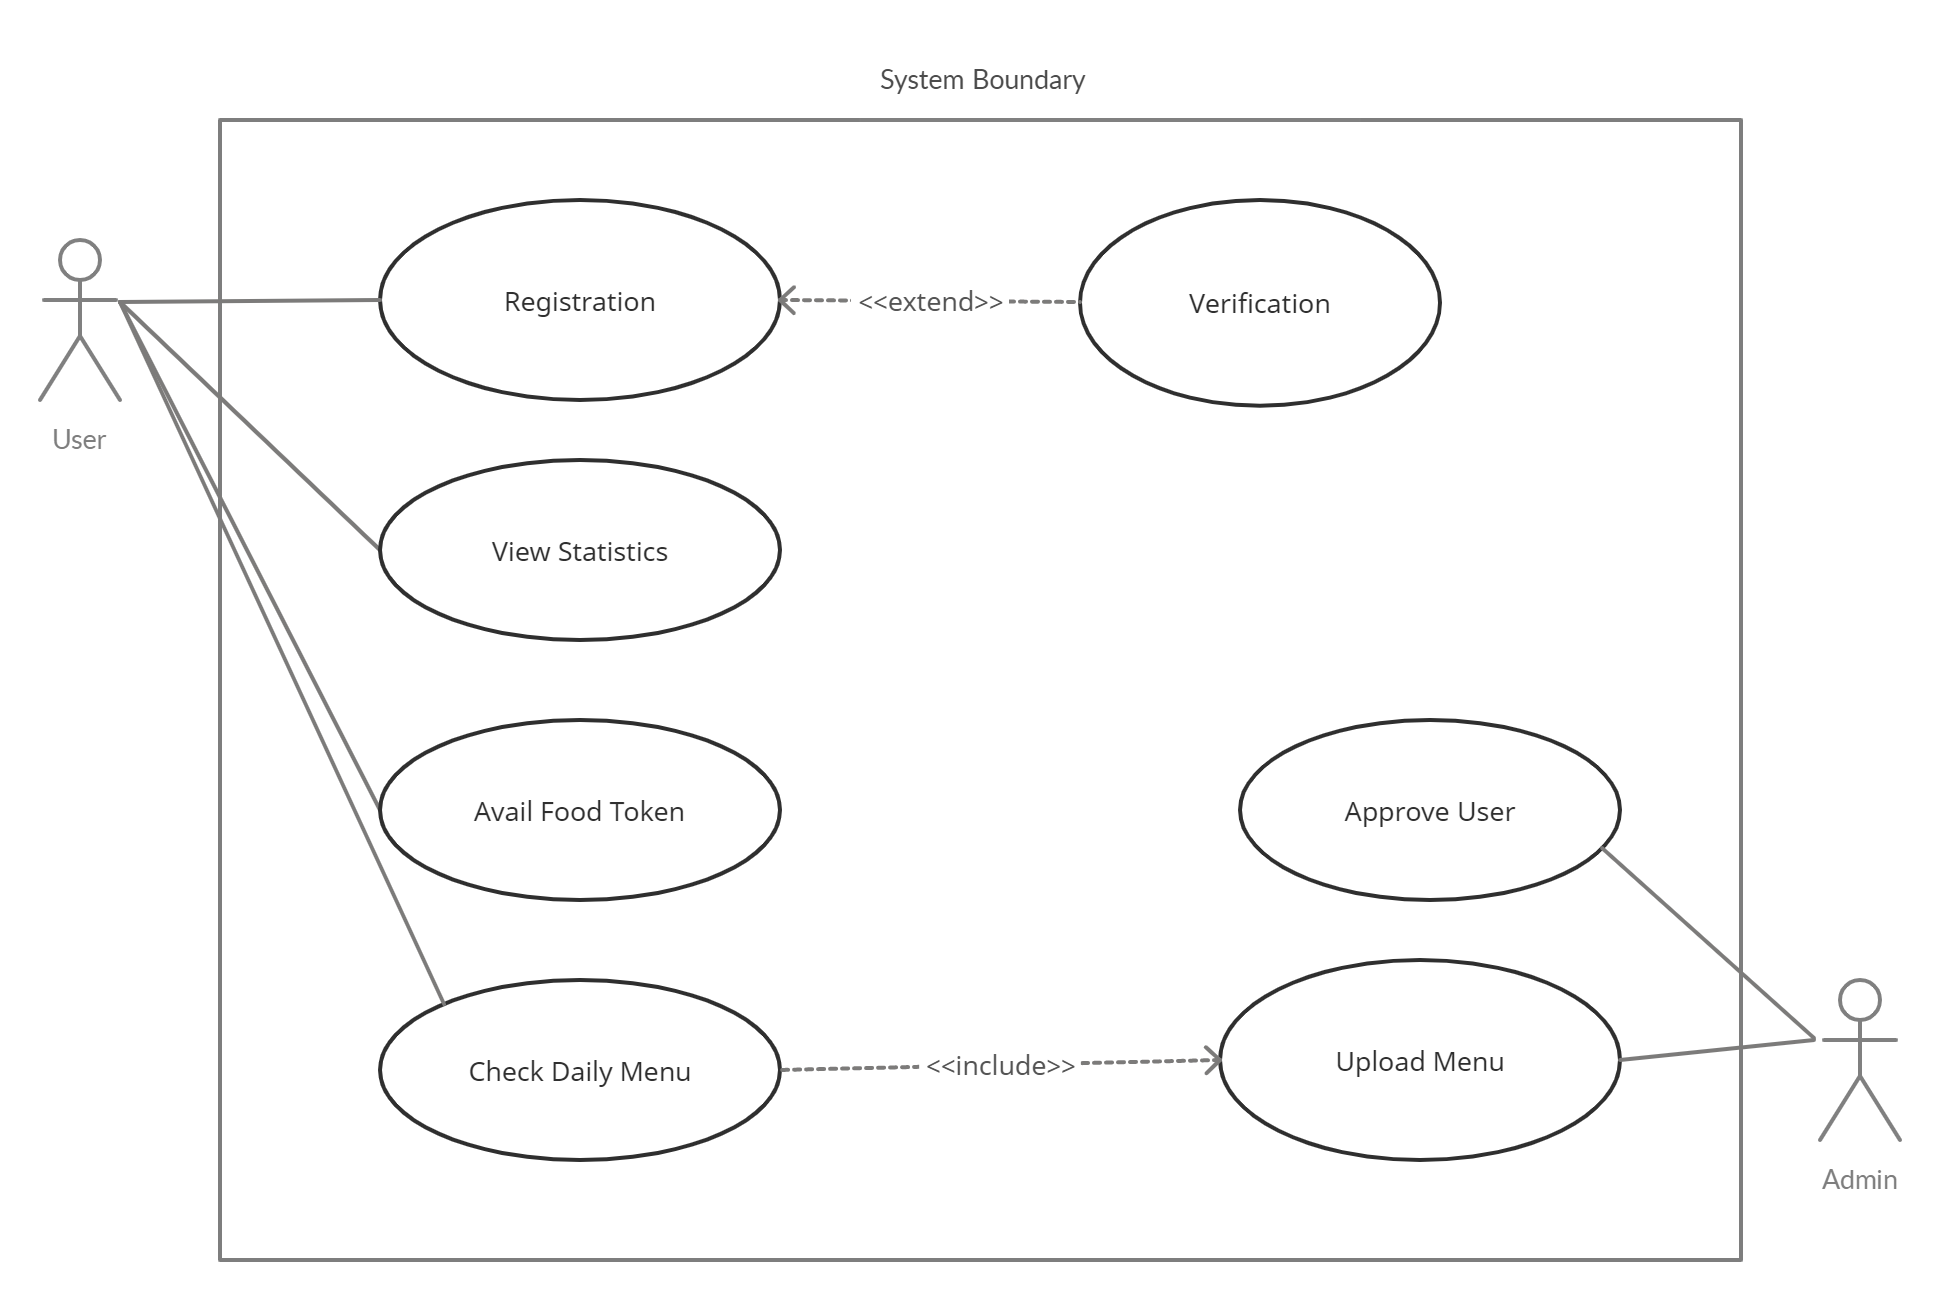
\includegraphics[width=0.7\linewidth]{usecase.jpg}
    \caption{Use Case Diagram}
\end{figure}

\begin{figure}[H]
    \centering
    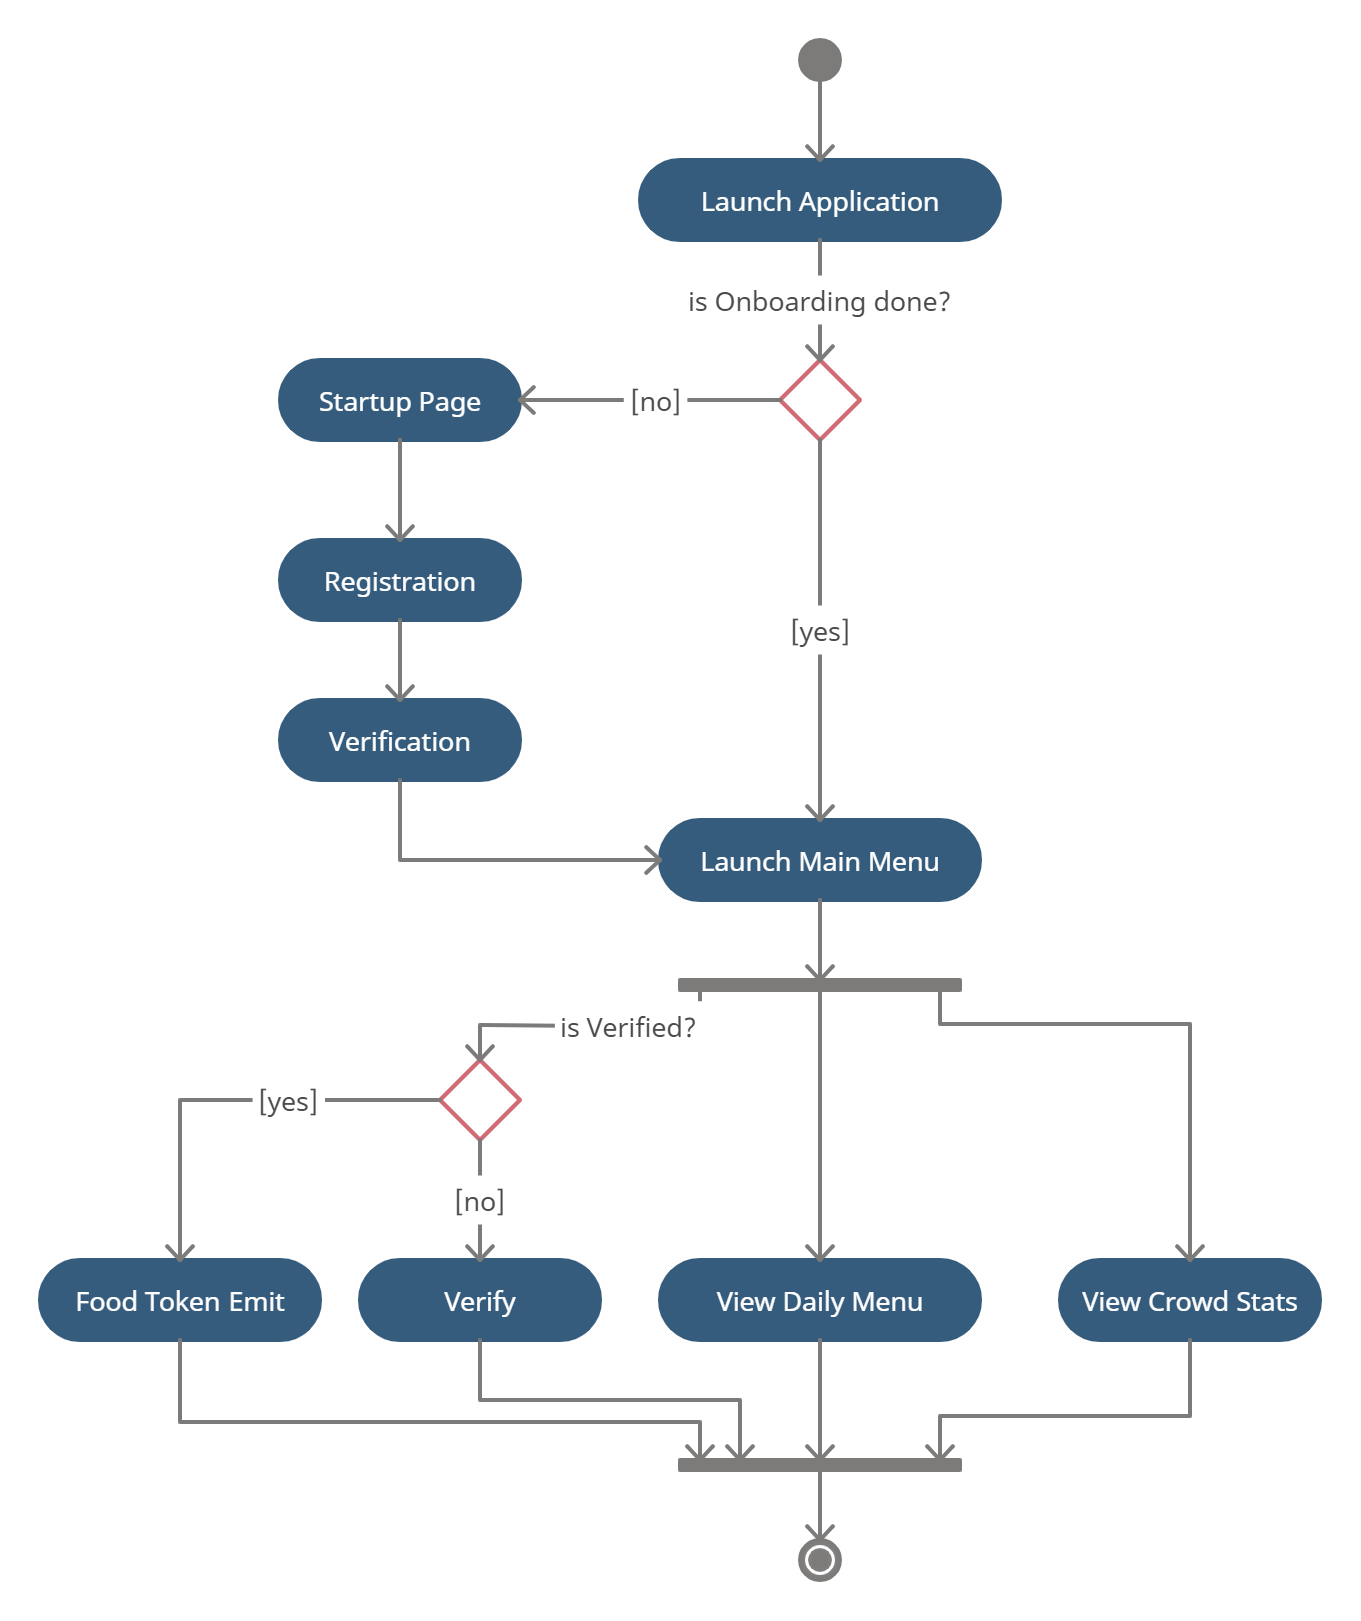
\includegraphics[width=0.7\linewidth]{activity.jpg}
    \caption{Activity Diagram}
\end{figure}
\newpage

% ---------------- UI Screenshots ----------------
\section*{\LARGE{UI Screenshots}}
\addcontentsline{toc}{section}{\protect\numberline{}UI Screenshots}

\begin{center}
    Main Splash Screen \\
    \vskip0.5cm
    \fbox{
\includegraphics[width=5cm]{landing.jpg}}
    \vskip1cm
    Onboarding Screens \\
    \vskip0.5cm
    \fbox{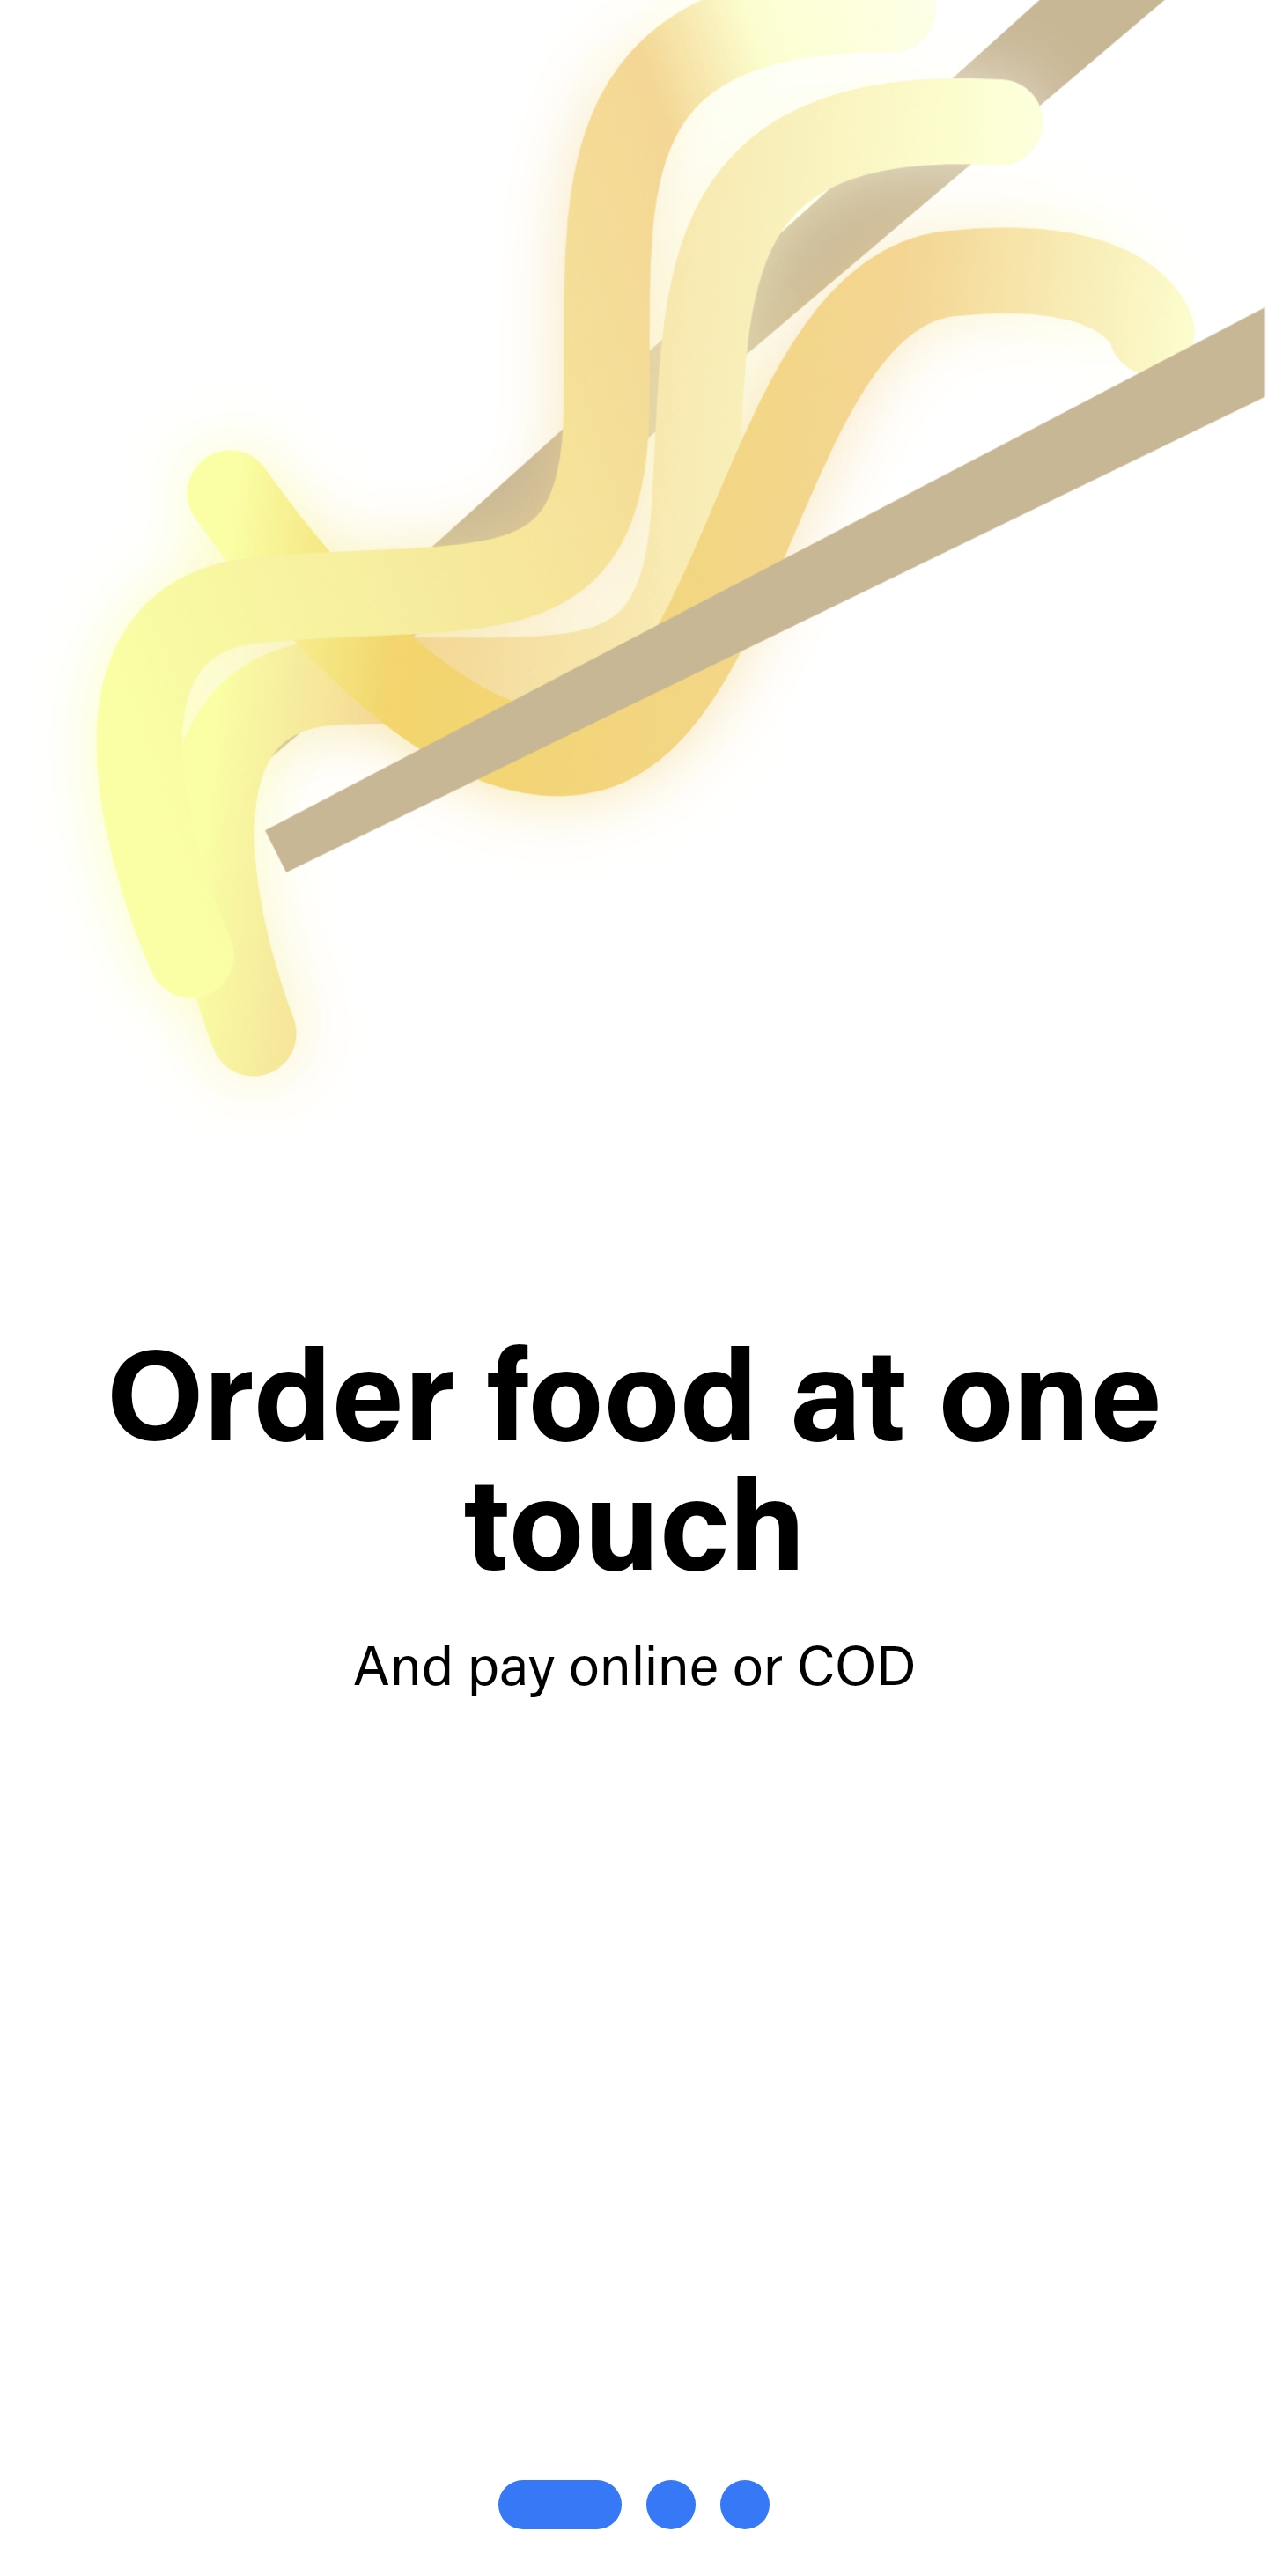
\includegraphics[width=5cm]{ob1.jpg}}\hspace{0.5cm}
    \fbox{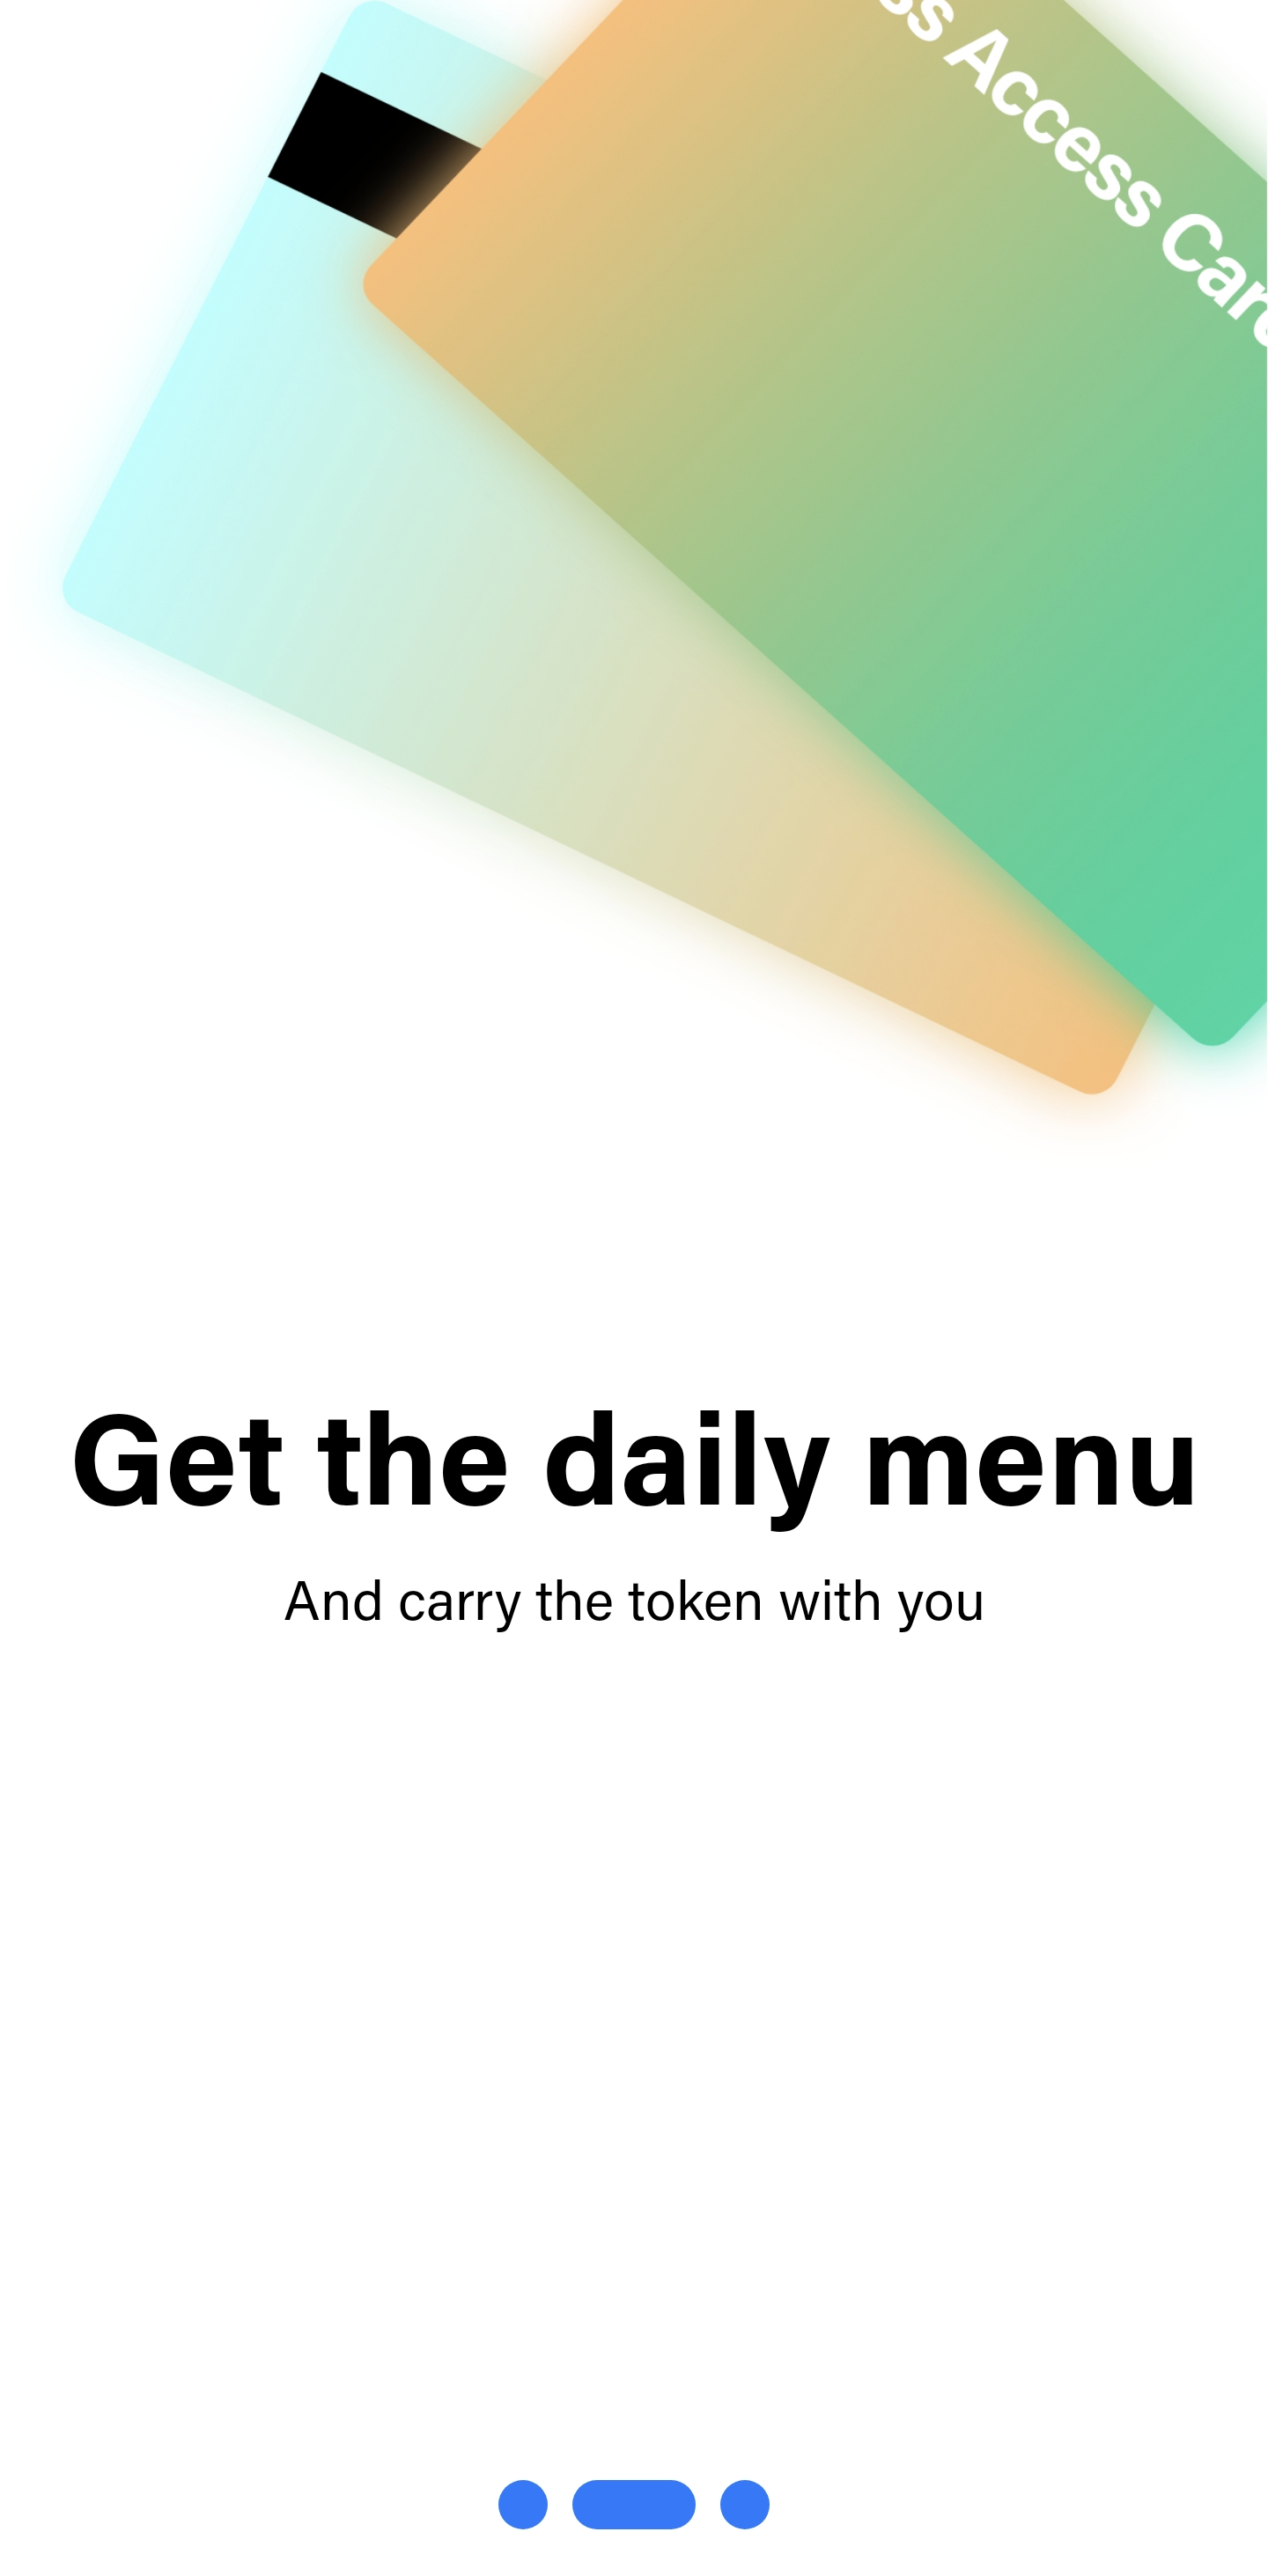
\includegraphics[width=5cm]{ob2.jpg}}\hspace{0.5cm}
    \fbox{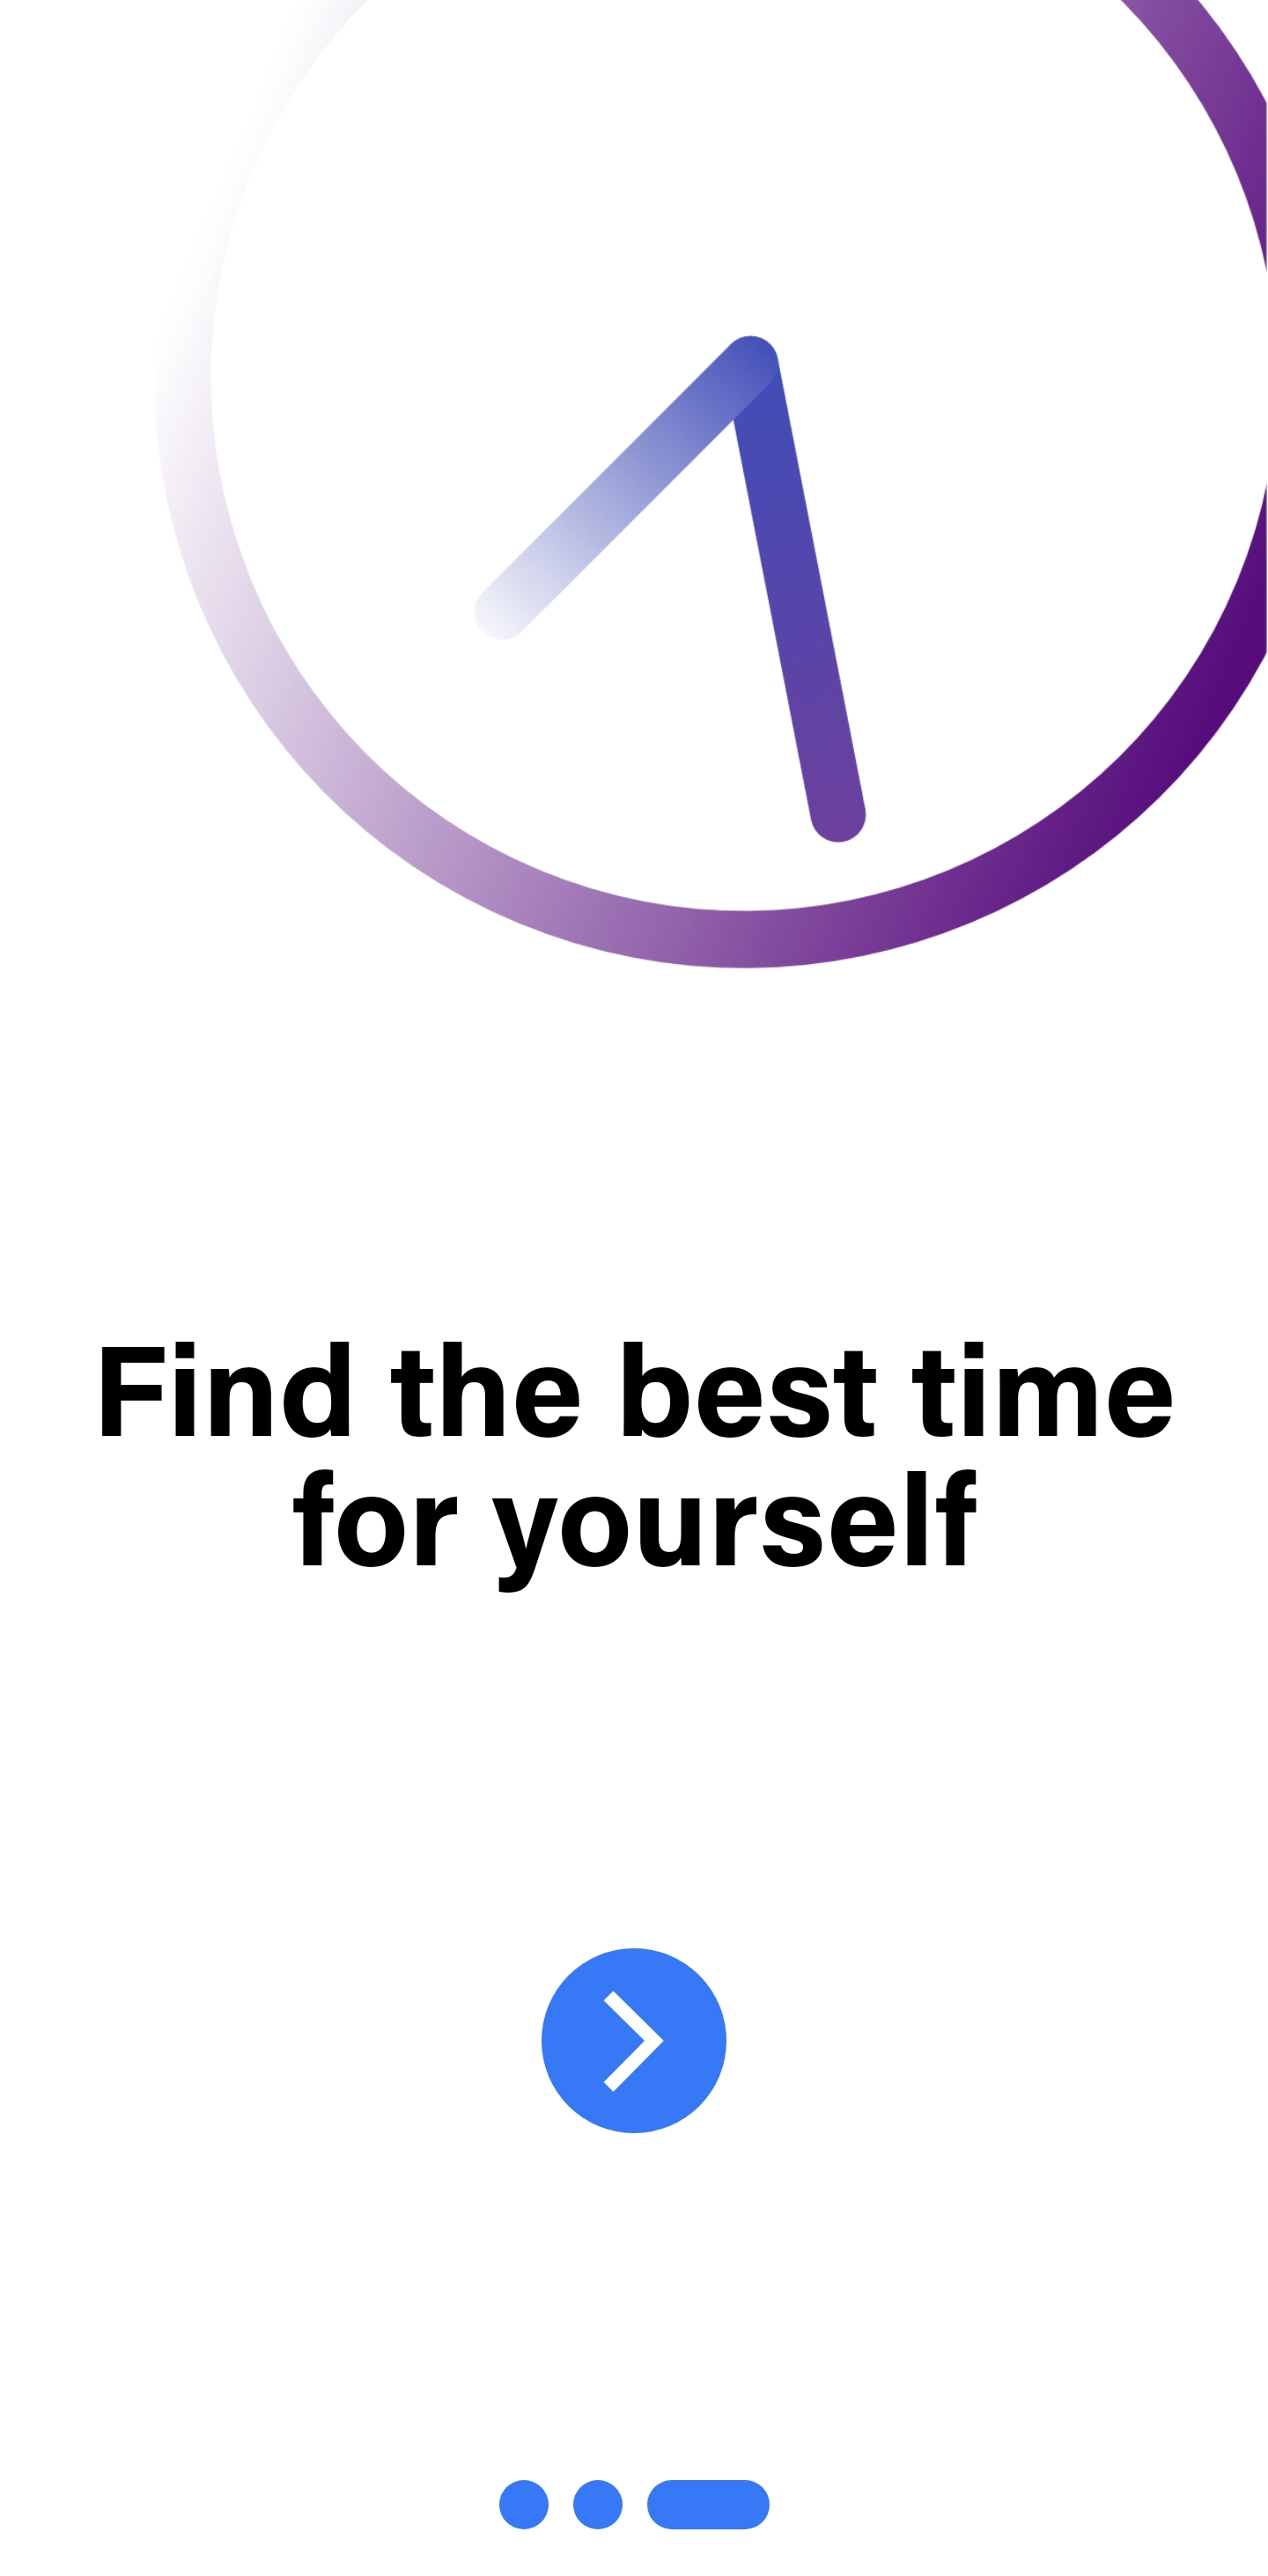
\includegraphics[width=5cm]{ob3.jpg}}
    \newpage
    Registration \& Verification Screens \\
    \vskip0.5cm
    \fbox{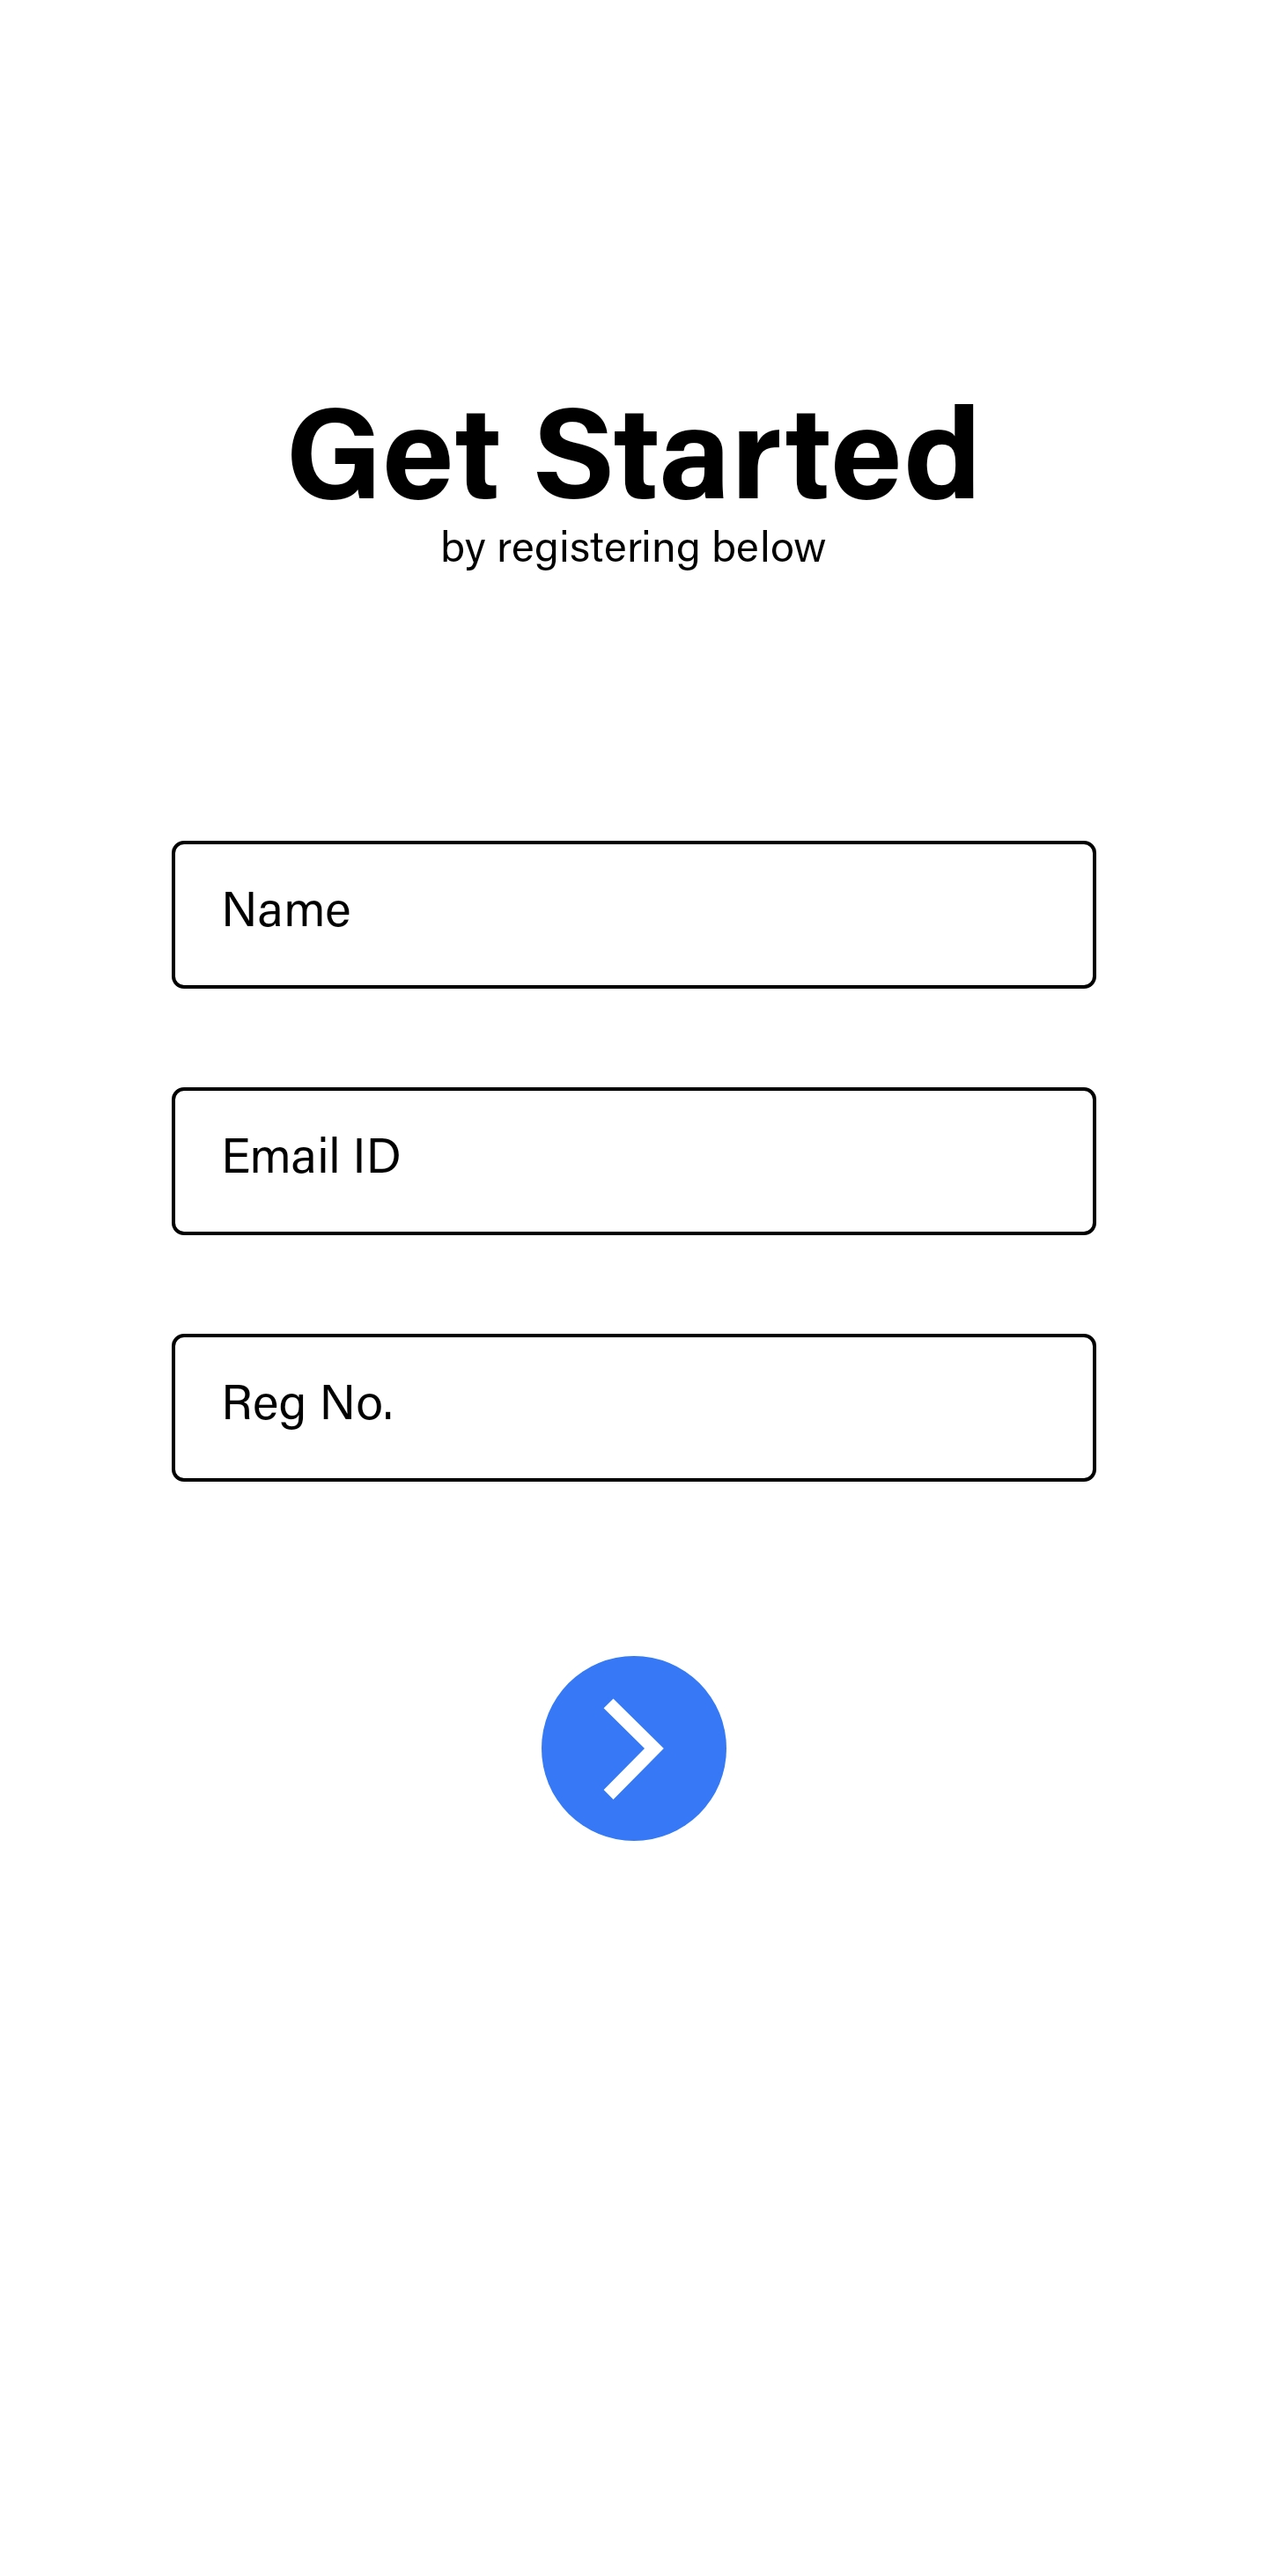
\includegraphics[width=5cm]{register.jpg}}\hspace{0.5cm}
    \fbox{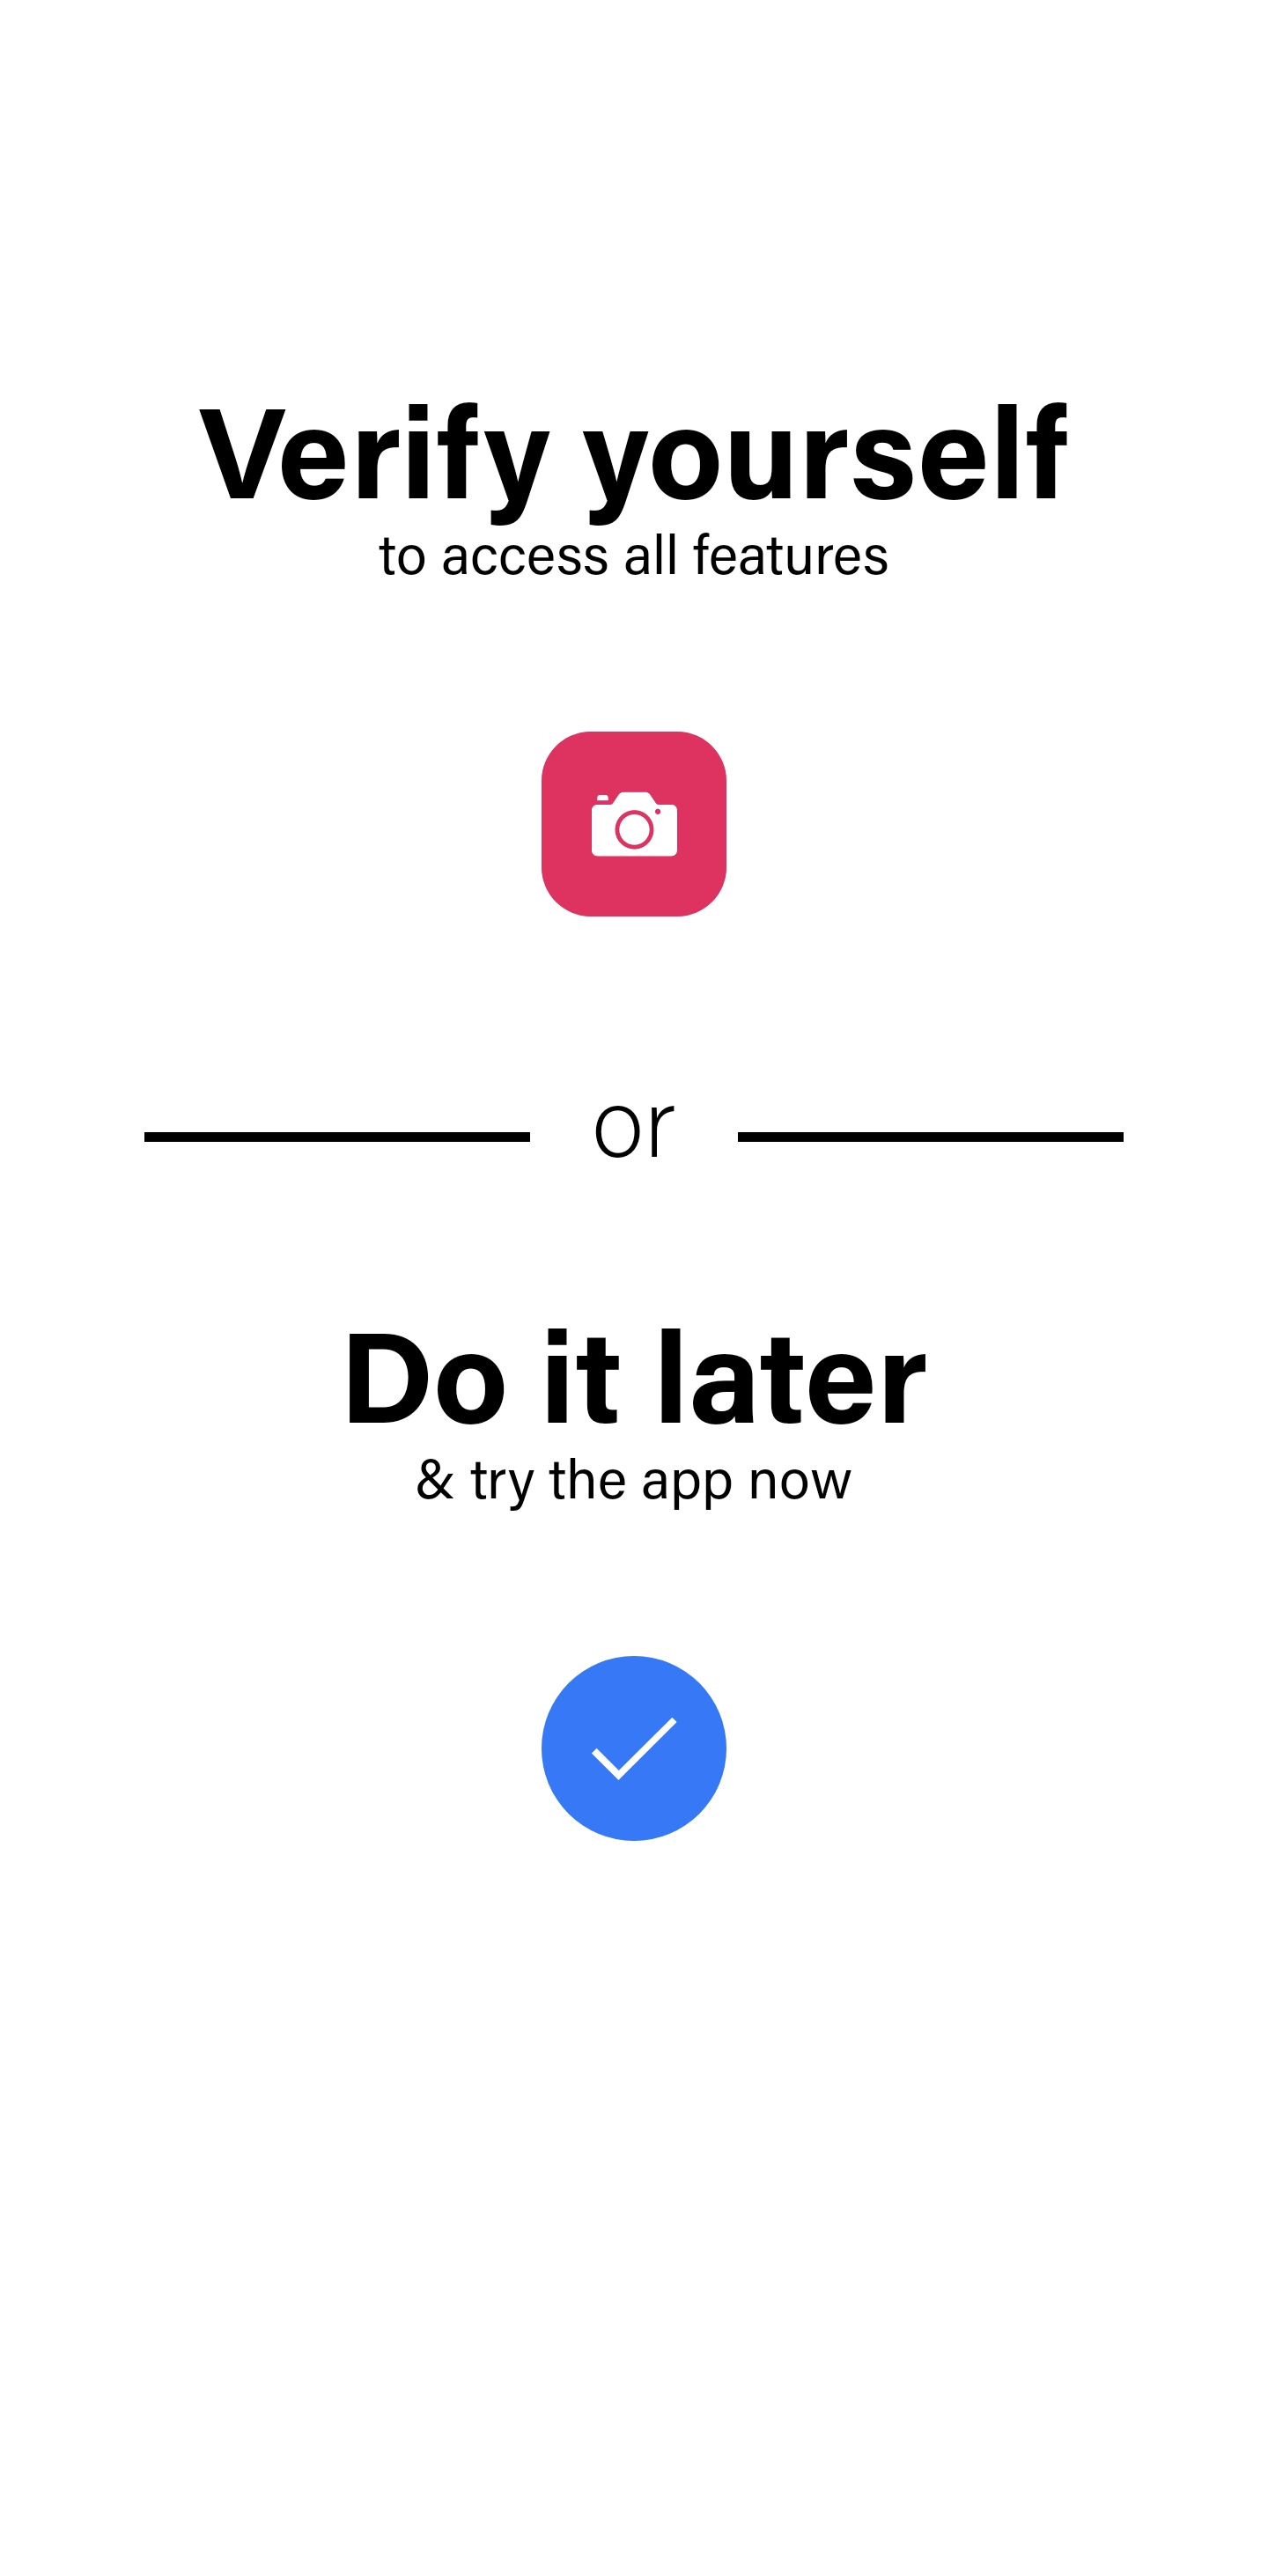
\includegraphics[width=5cm]{verify.jpg}}
    \vskip1cm
    Main Screen
    \vskip0.5cm
    \fbox{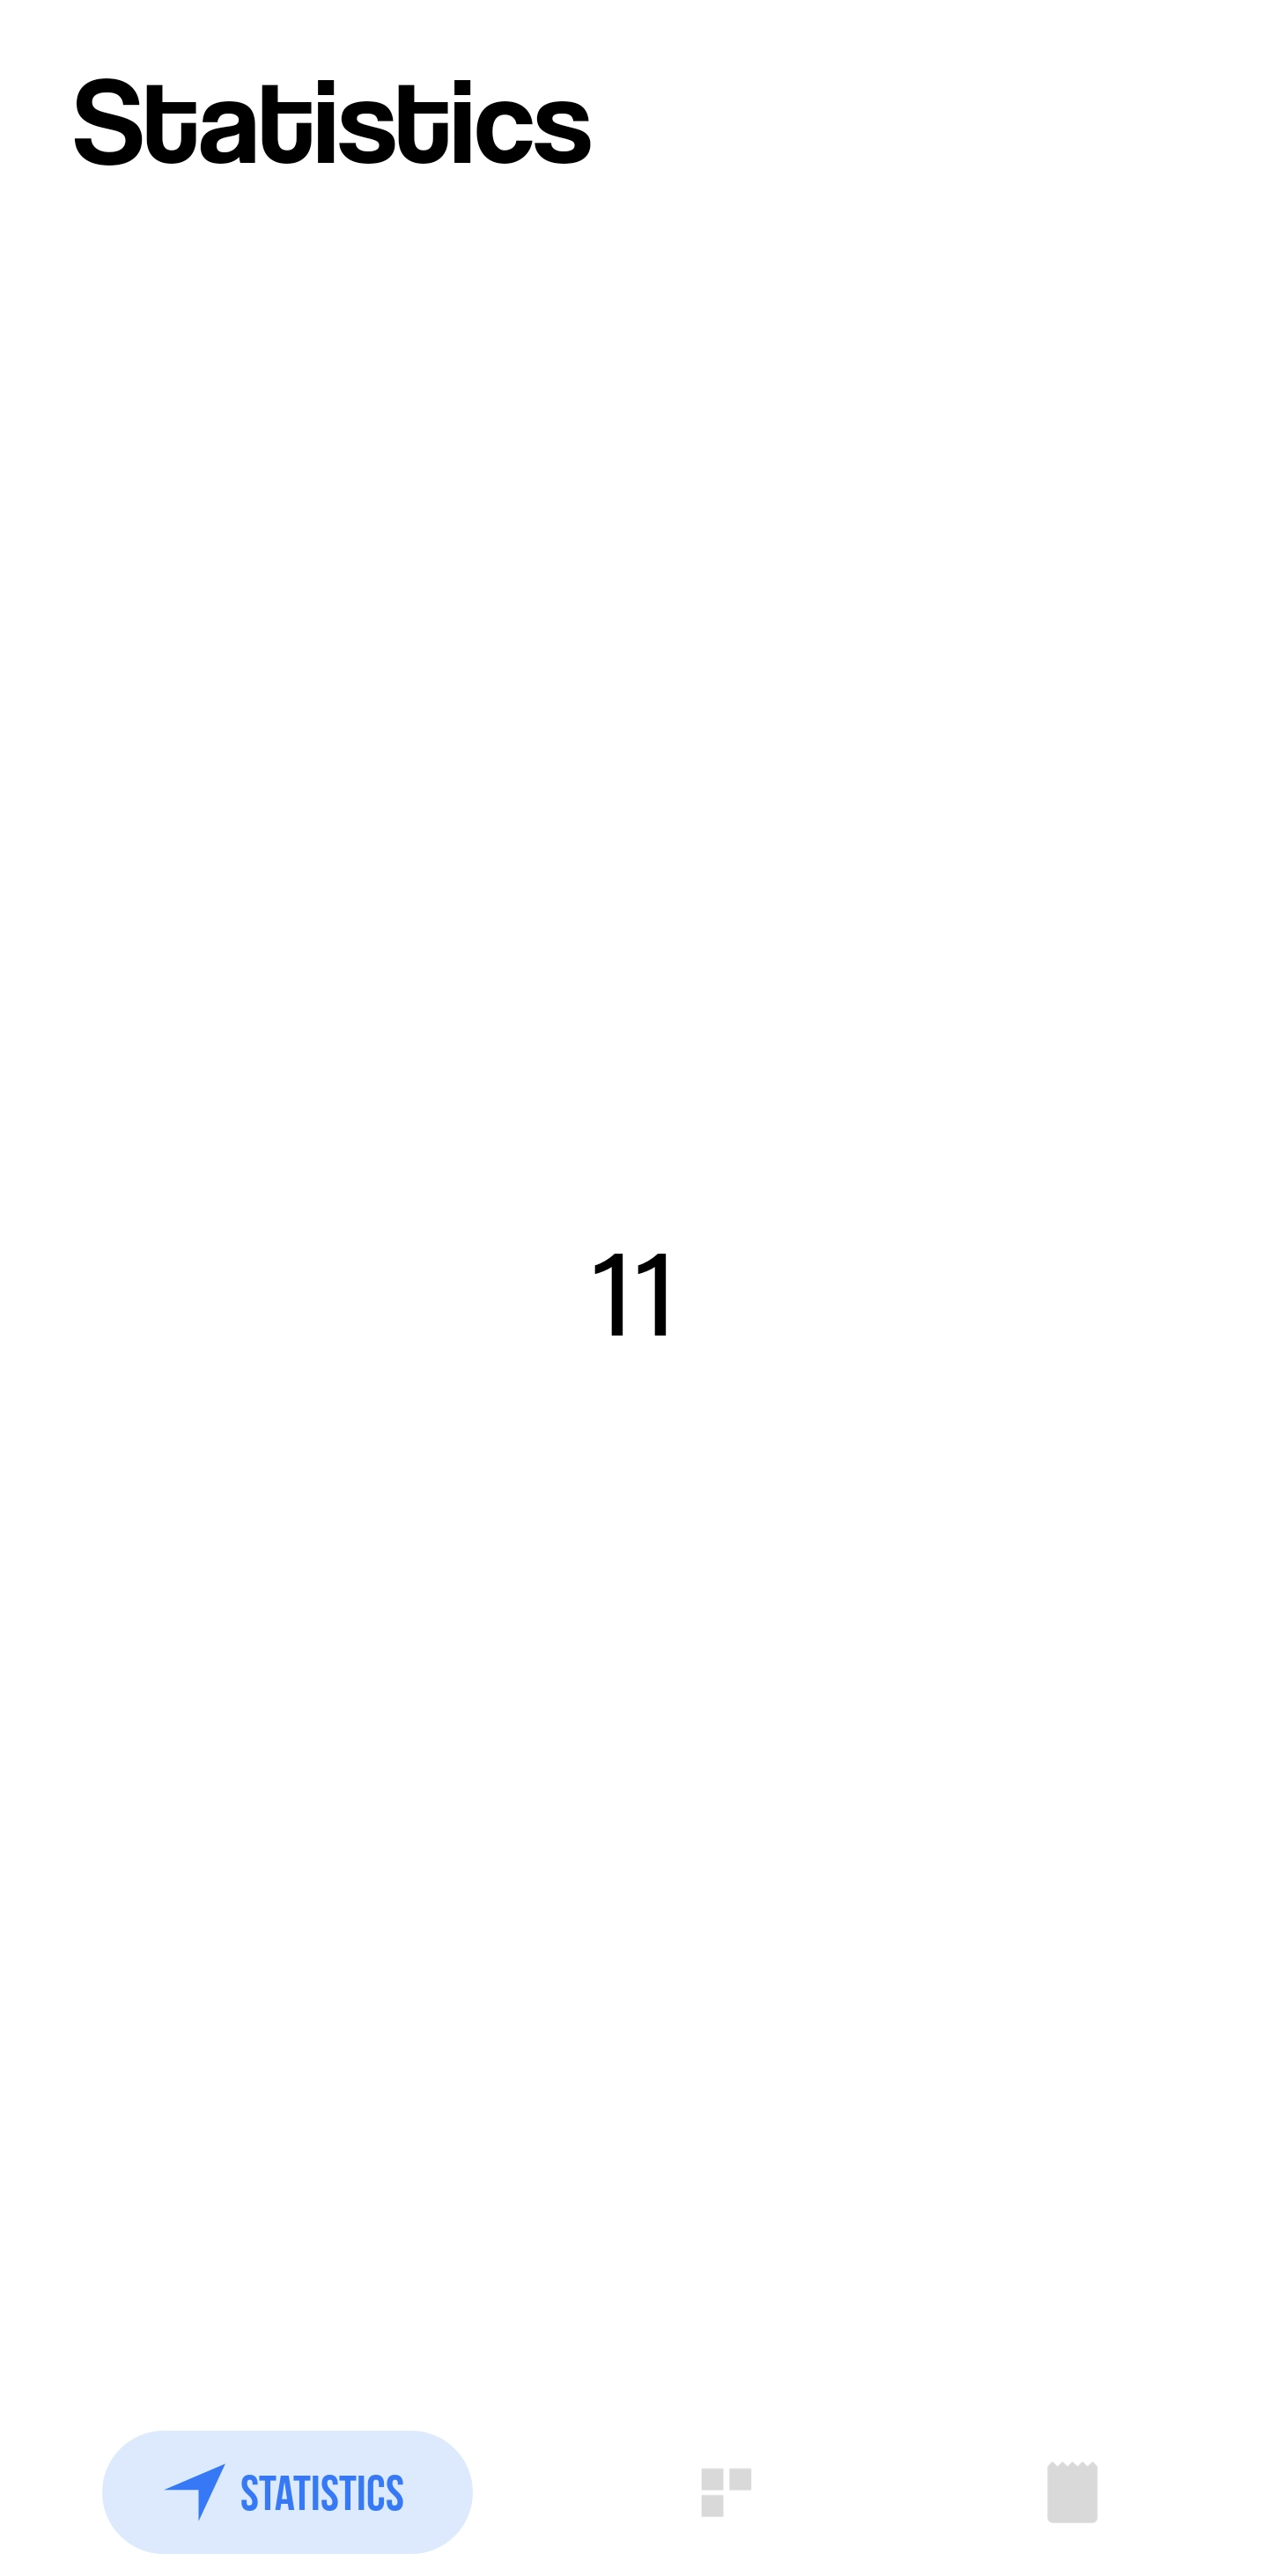
\includegraphics[width=5cm]{geofence.jpg}}\hspace{0.5cm}
    \fbox{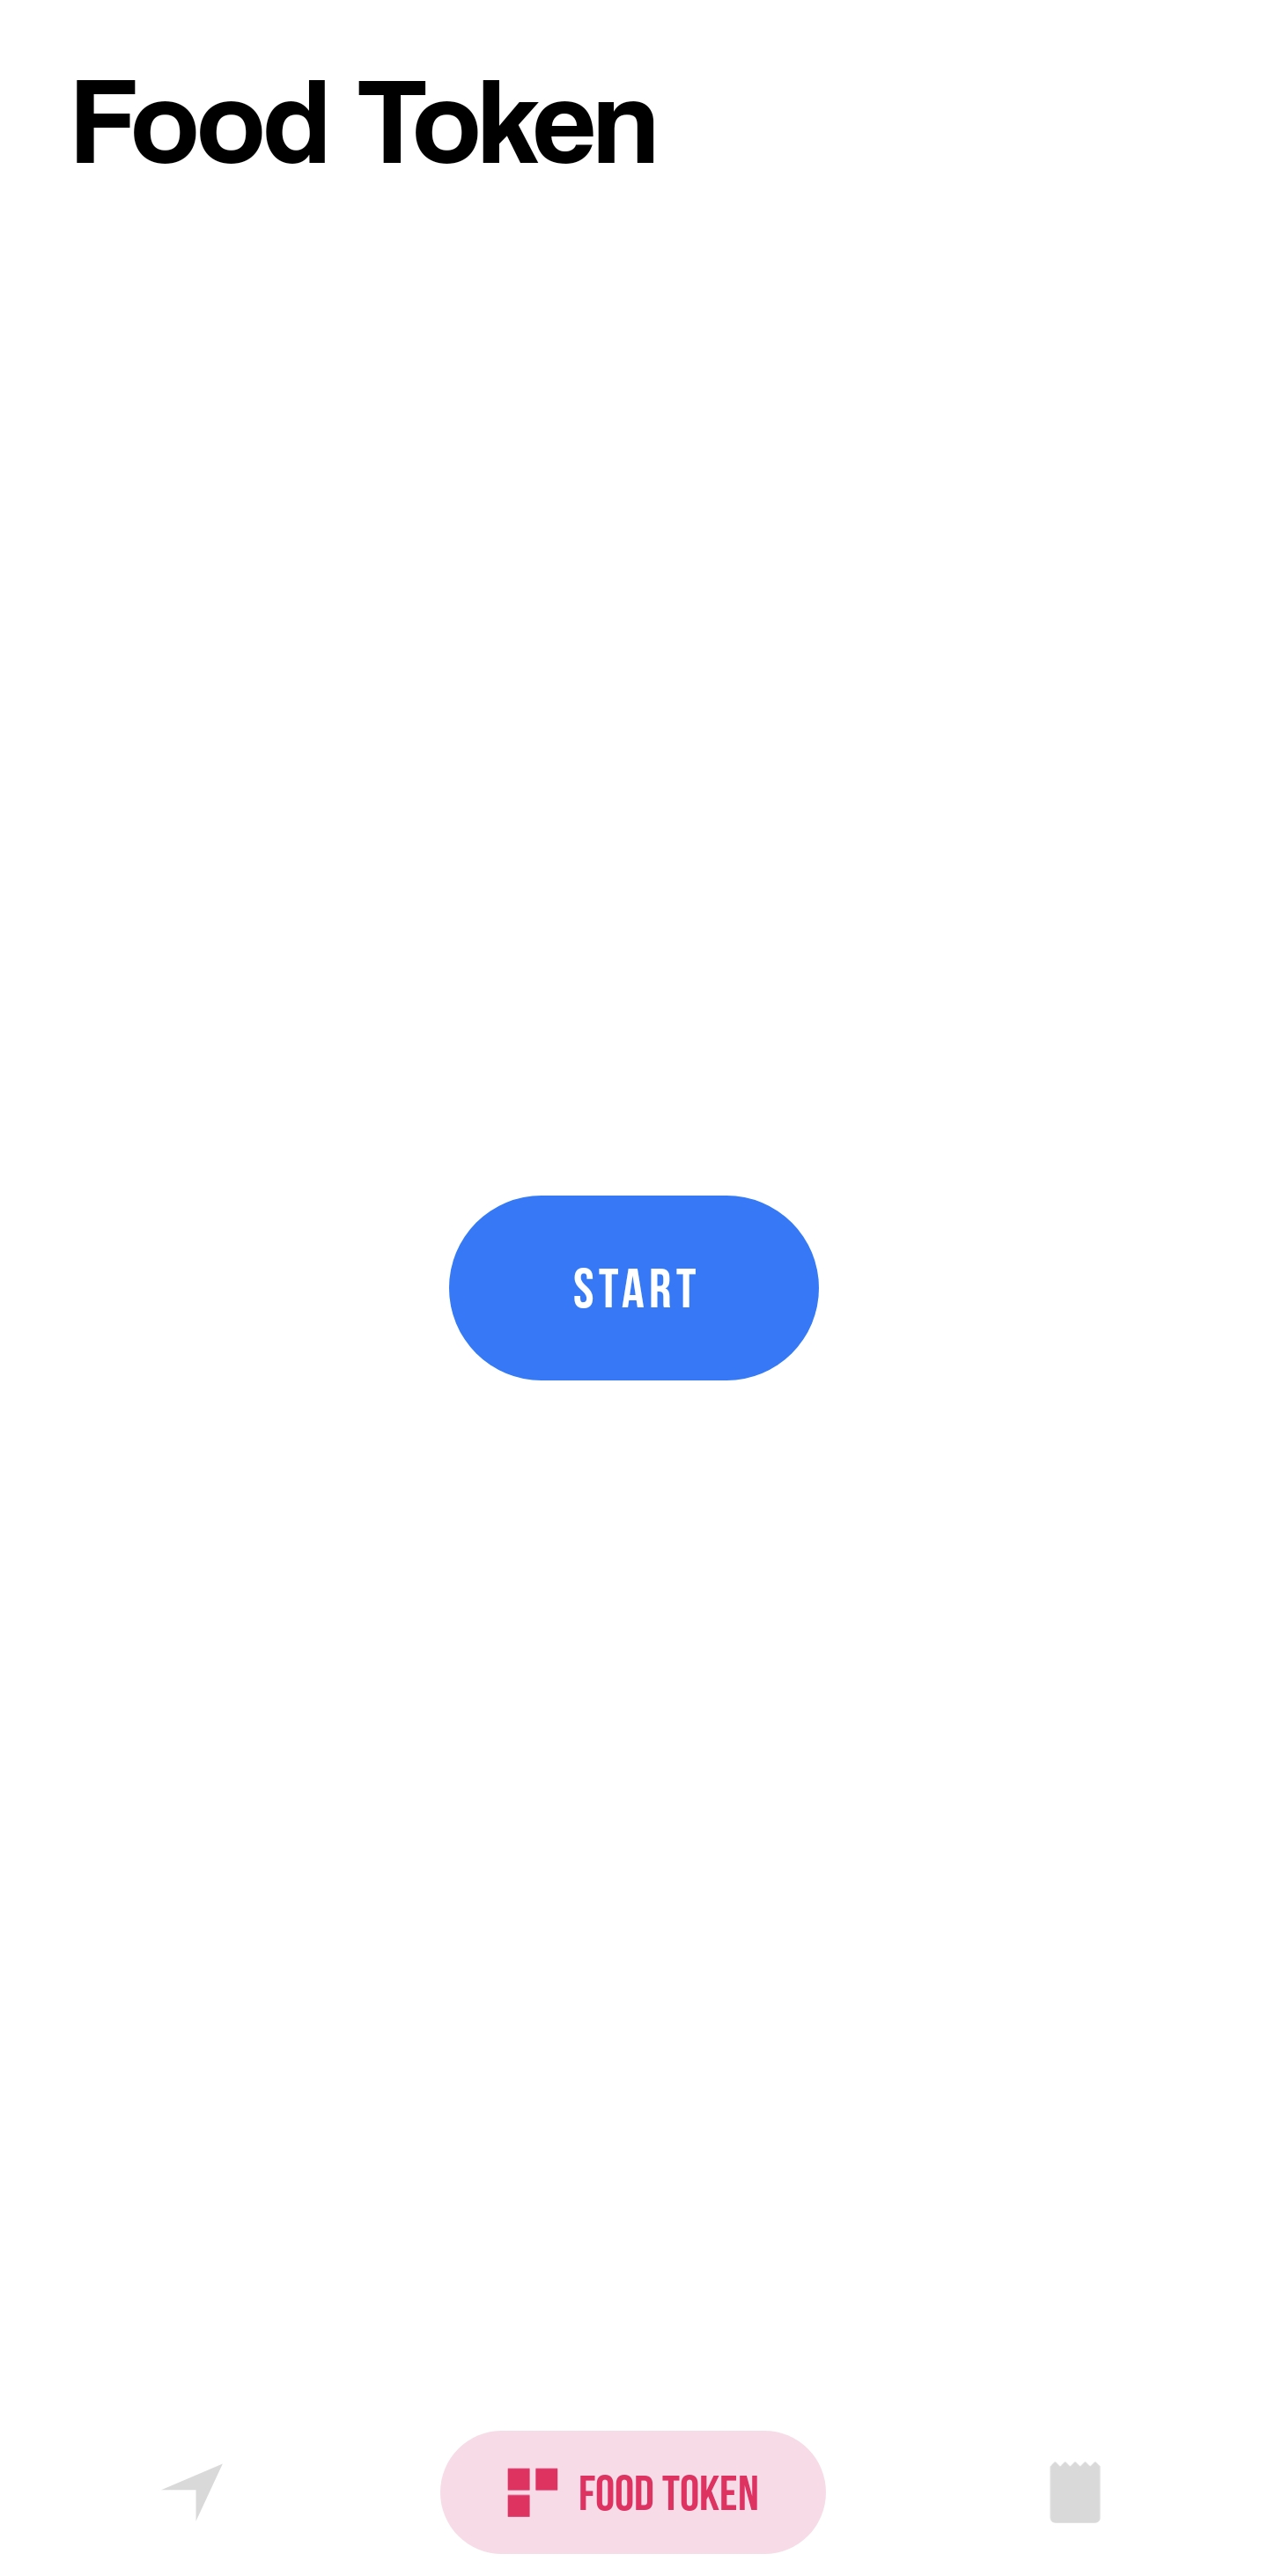
\includegraphics[width=5cm]{foodtoken.jpg}}\hspace{0.5cm}
    \fbox{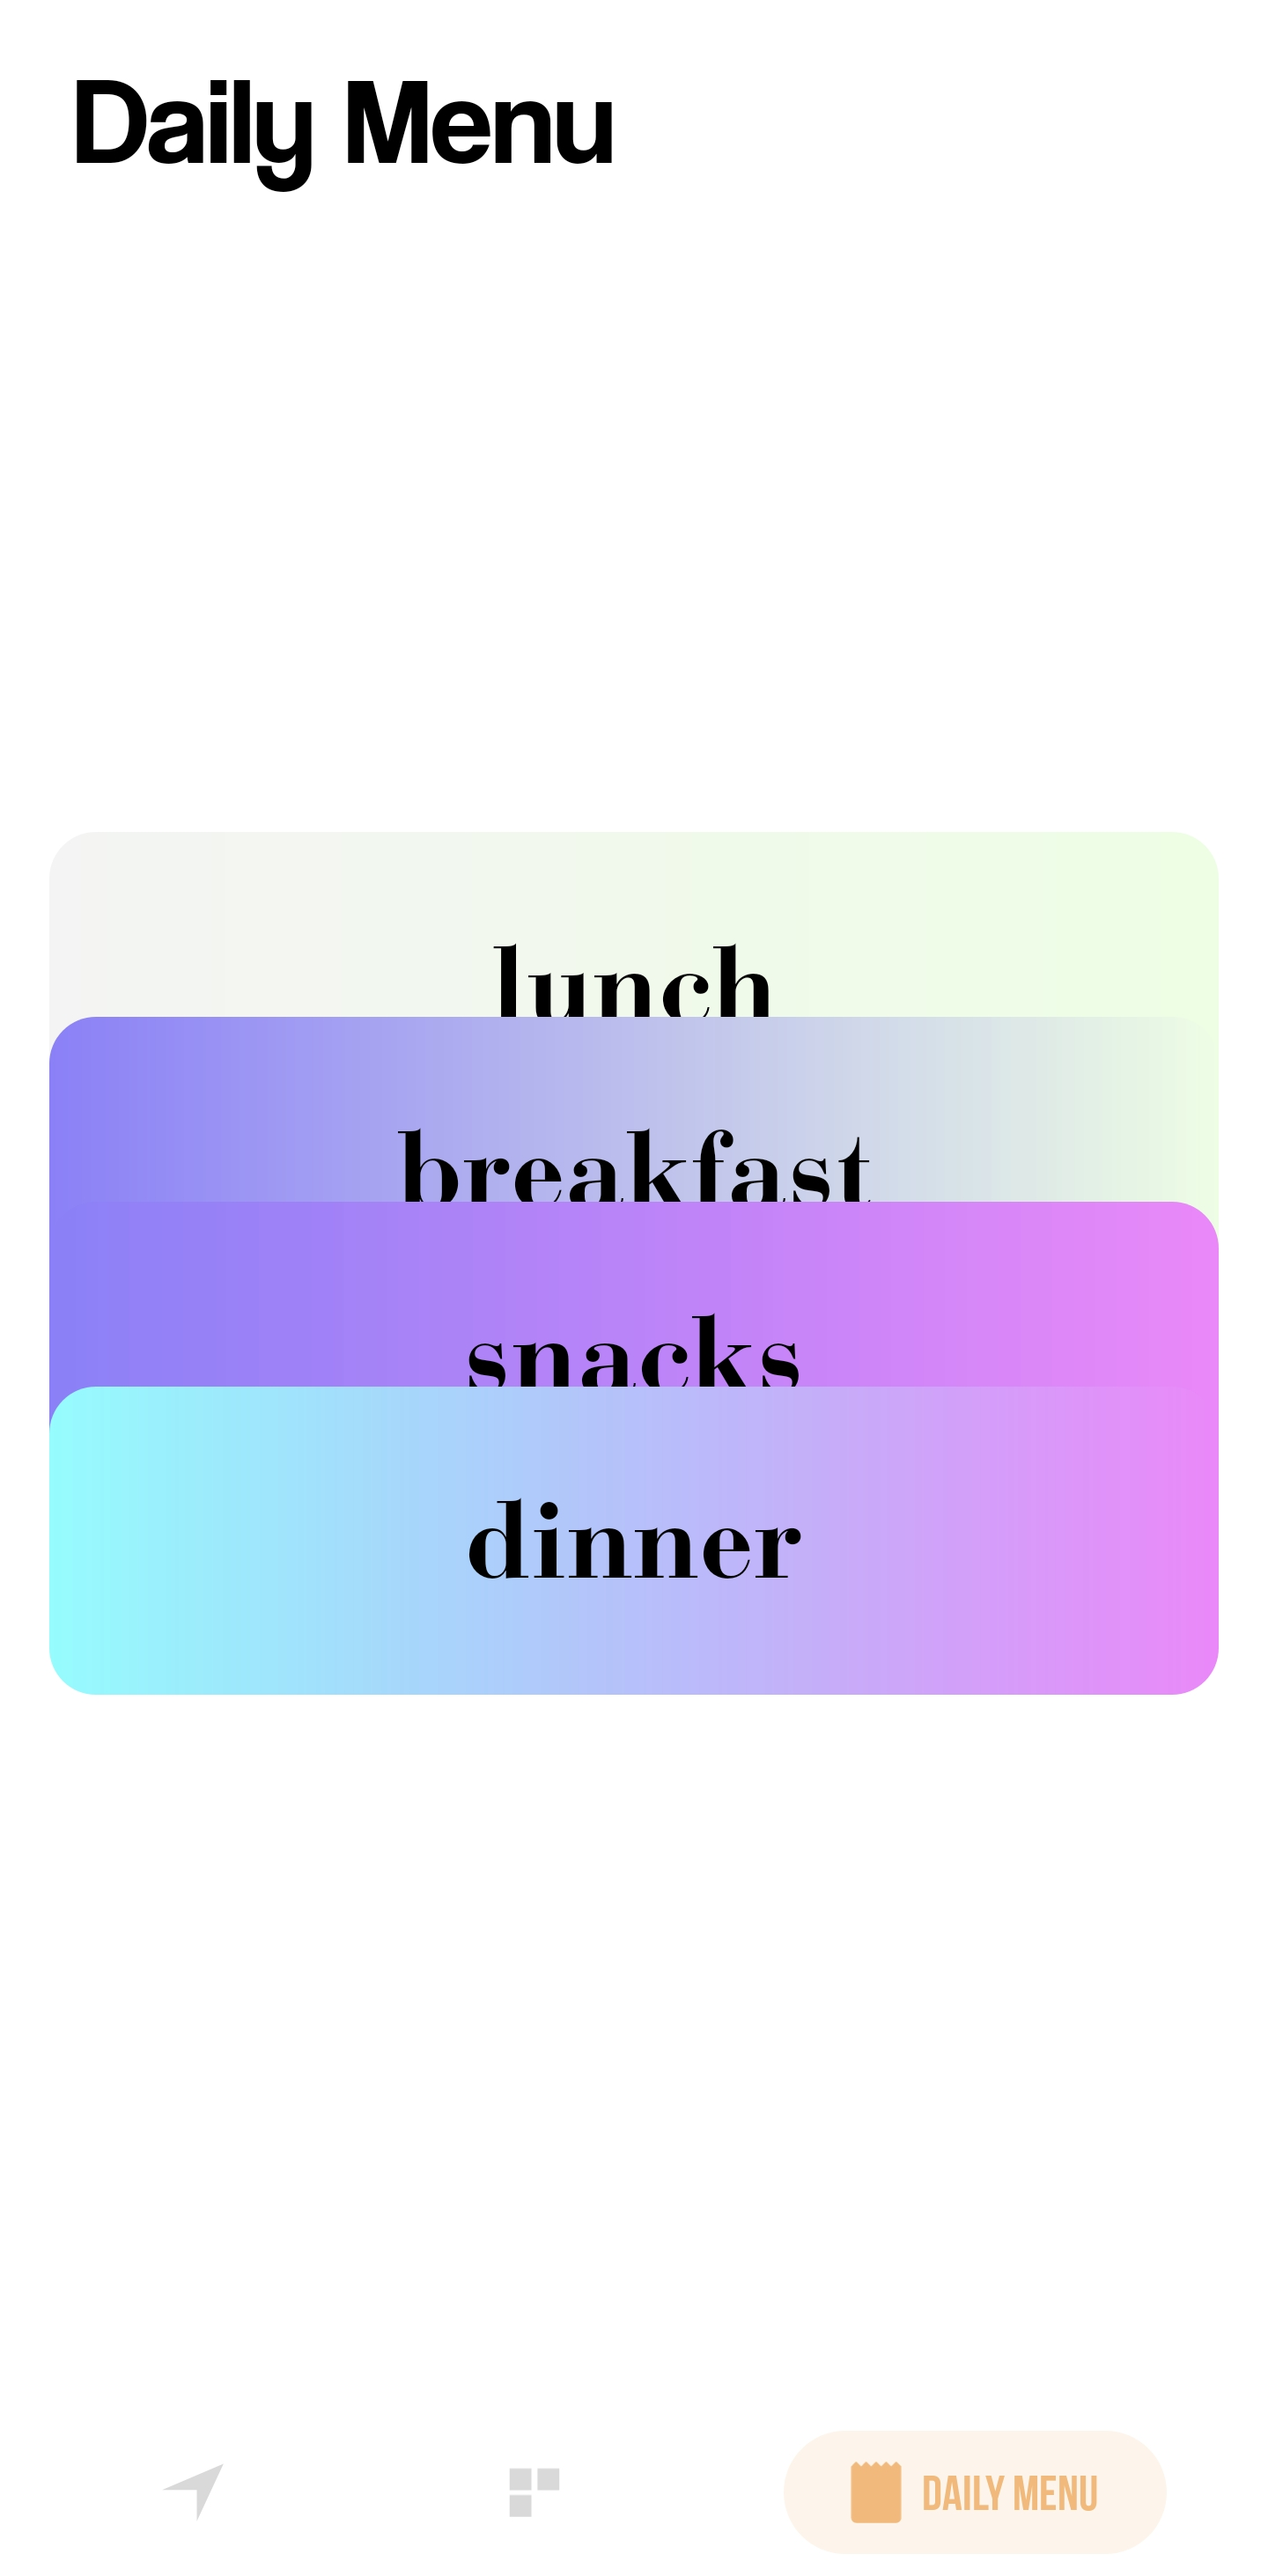
\includegraphics[width=5cm]{dailymenu.jpg}}
\end{center}
\newpage

% ---------------- Results ----------------
\section*{\LARGE{Results}}
\addcontentsline{toc}{section}{\protect\numberline{}Results}

{\justify
Thus we have implemented the following \fbox{\href{https://drive.google.com/file/d/1JFDdxTUJtG8xZVHFdeNY84Cx3PckzsT5/view?usp=drivesdk}{\textbf{App Demo}}} \& \fbox{\href{https://github.com/nikeplusdash/FC2/}{\textbf{Repo}}} \footnote{other functional components will be explained in PPT}
\vskip0.2cm
We have managed to achieve the following objectives:

\begin{enumerate}
\item A prototype of NFC Food Token to show the use case of Virtual Token over an application. Due to limitation of hardware, complete food token emulation could not be achieved;
\item Geofencing to gather crowd statistics
\item A pretty and minimal UI for faster usage
\item Verification using AI/ML
\end{enumerate}}

% ---------------- Conclusion ----------------
\section*{\LARGE{Conclusion}}
\addcontentsline{toc}{section}{\protect\numberline{}Conclusion}

{\justify
The application proves itself useful especially at the time of the pandemic, due to crowd control and virtual token system which help one to adhere to pandemic rules and also save your time and as the saying goes, time is money but this time you own it. This app is an environment-friendly initiative as the virtual token allows us to cut down on plastic \gls{RFID} cards and any loss of it as well. Moreover, the daily menu saves paper spent on printing the menu. These benefits are not only eco-friendly but also very economical as well. All these aside, the app features a minimal and neat UI that is easily navigable.
}

% ---------------- Future Work ----------------
\section*{\LARGE{Future Work}}
\addcontentsline{toc}{section}{\protect\numberline{}Future Work}

{\justify
Possible extensions to the app are feasible

\begin{itemize}
\item Predict food menu preference \& crowding correlation to improve efficiency of the mess
\item Using crowd data and dwell timings to provide weekly crowding statistics
\item Implementation of Host-Card Emulation for better faciliation of food tokens
\item An ordering service feature
\item UPI Payment Integration for buying food tokens temporarily or for ordering
\item Using ML for recognising user from user\textquotesingle s picture in Identity Card
\end{itemize}
}

% ---------------- References ----------------
\section*{\LARGE{References}}
\addcontentsline{toc}{section}{\protect\numberline{}References}
\begin{thebibliography}{widest entry} 
\bibitem[1]{picasso} \url{https://square.github.io/picasso/}
\bibitem[2]{dotsindicator} \url{https://github.com/tommybuonomo/dotsindicator}
\bibitem[3]{bubbletab} \url{https://github.com/akshay2211/BubbleTabBar}
\bibitem[4]{cardstack} \url{https://github.com/loopeer/CardStackView}
\bibitem[5]{firebase} \url{https://firebase.google.com/}
\end{thebibliography}   
\end{document}